\documentclass[11pt]{book}

\usepackage{cmap}

\usepackage[russian,english]{babel}
\usepackage[T2A]{fontenc}
\usepackage[default]{sourcesanspro}

\usepackage{ifthen}

\usepackage{amsmath}
\usepackage{listings}
\usepackage{epigraph}
\usepackage{url}
\usepackage[cm]{fullpage}
\usepackage{graphicx}
\usepackage{framed}
\usepackage{color}
\usepackage{float}
\usepackage{tikz}
\usetikzlibrary{arrows}
\usepackage[nottoc]{tocbibind}
%\usepackage{esint}
%\usepackage{charter}
%\usepackage[charter]{mathdesign}
\usepackage[footnote,printonlyused,withpage]{acronym}
\usepackage[]{hyperref} % should be last

%\definecolor{lstbgcolor}{rgb}{0.94,0.94,0.94}
\definecolor{lstbgcolor}{rgb}{1,1,1}

\newcommand{\TT}[1]{\texttt{#1}}

\newcommand{\TITLE}{Mathematics for programmers (early draft)}
\newcommand{\AUTHOR}{Dennis Yurichev \TT{<dennis(@)yurichev.com>}}

\hypersetup{
    pdftex,
    colorlinks=true,
    allcolors=blue,
    pdfauthor={\AUTHOR},
    pdftitle={\TITLE},
    pdfpagemode=None
}

\iffalse
\lstset{
    backgroundcolor=\color{lstbgcolor},
    basicstyle=\ttfamily, 
    breaklines=true,
    frame=single,
    columns=fullflexible,keepspaces,
}
\fi

\lstset{
    %backgroundcolor=\color{lstbgcolor},
    %backgroundcolor=\color{light-gray},
    %basicstyle=\ttfamily\small,
    basicstyle=\ttfamily\normalsize,
    %basicstyle=\ttfamily\large,
    %basicstyle=\ttfamily\footnotesize,
    literate={~} {$\sim$}{1},
    breaklines=true,
    frame=single,
    %columns=fullflexible,keepspaces,
    columns=keepspaces,
    escapeinside=§§,
    inputencoding=utf8
}

\author{\AUTHOR}
\title{\TITLE}
%\date{August-2015 --- ...}

\definecolor{digits}{RGB}{0,0,0}
\definecolor{colkw}{RGB}{0,0,0}

%\definecolor{colstr}{RGB}{80,80,80}
%\definecolor{colid}{RGB}{80,80,80}

\definecolor{colstr}{RGB}{0,0,0}
\definecolor{colid}{RGB}{0,0,0}

\definecolor{colcomment}{RGB}{130,130,130}
%\definecolor{colcomment}{RGB}{170,170,170}

\definecolor{colbg}{RGB}{255,255,255}

\lstdefinestyle{custompy}{
  language=Python,
  showstringspaces=false,
  backgroundcolor=\color{colbg},
  keywordstyle=\color{colkw},
  commentstyle=\color{colcomment},
  identifierstyle=\color{colid},
  stringstyle=\color{colstr}
}

\lstdefinestyle{customc}{
  language=C,
  showstringspaces=false,
  backgroundcolor=\color{colbg},
  keywordstyle=\color{colkw},
  commentstyle=\color{colcomment},
  identifierstyle=\color{colid},
  stringstyle=\color{colstr}
}

% https://tex.stackexchange.com/questions/5148/how-can-i-change-the-font-size-in-math-equations
% \DeclareMathSizes{12}{12}{12}{12}

\begin{document}

% reworked from http://tex.stackexchange.com/questions/26181/create-context-sensitive-headings

\newcommand{\currentlevel}{}

\newcommand{\leveldown}%
{   
    \ifthenelse{\equal{\currentlevel}{sp}}%
    {\renewcommand{\currentlevel}{sp}}{}%    
    \ifthenelse{\equal{\currentlevel}{p}}%
    {\renewcommand{\currentlevel}{sp}}{}%    
    \ifthenelse{\equal{\currentlevel}{sss}}%
    {\renewcommand{\currentlevel}{p}}{}%    
    \ifthenelse{\equal{\currentlevel}{ss}}%
    {\renewcommand{\currentlevel}{sss}}{}%    
    \ifthenelse{\equal{\currentlevel}{s}}%
    {\renewcommand{\currentlevel}{ss}}{}%
    \ifthenelse{\equal{\currentlevel}{c}}%
    {\renewcommand{\currentlevel}{s}}{}%
}

\newcommand{\levelup}%
{
    \ifthenelse{\equal{\currentlevel}{c}}%
    {\renewcommand{\currentlevel}{c}}{}%
    \ifthenelse{\equal{\currentlevel}{s}}%
    {\renewcommand{\currentlevel}{c}}{}%
    \ifthenelse{\equal{\currentlevel}{ss}}%
    {\renewcommand{\currentlevel}{s}}{}%
    \ifthenelse{\equal{\currentlevel}{sss}}%
    {\renewcommand{\currentlevel}{ss}}{}
    \ifthenelse{\equal{\currentlevel}{p}}%
    {\renewcommand{\currentlevel}{sss}}{}
    \ifthenelse{\equal{\currentlevel}{sp}}%
    {\renewcommand{\currentlevel}{p}}{}%
}

\newcommand{\myheading}[1]%
{   \ifthenelse{\equal{\currentlevel}{c}}%
    {\chapter{#1}}{}%
    \ifthenelse{\equal{\currentlevel}{s}}%
    {\section{#1}}{}%
    \ifthenelse{\equal{\currentlevel}{ss}}%
    {\subsection{#1}}{}%
    \ifthenelse{\equal{\currentlevel}{sss}}%
    {\subsubsection{#1}}{}%
    \ifthenelse{\equal{\currentlevel}{p}}%
    {\myparagraph{#1}}{}%
    \ifthenelse{\equal{\currentlevel}{sp}}%
    {\mysubparagraph{#1}}{}%
}

\newcommand{\newchapter}[1]{\chapter{#1}\renewcommand{\currentlevel}{c}}
\newcommand{\newsection}[1]{\section{#1}\renewcommand{\currentlevel}{s}}
\newcommand{\newsubection}[1]{\subsection{#1}\renewcommand{\currentlevel}{ss}}
\newcommand{\newsubsubection}[1]{\subsubsection{#1}\renewcommand{\currentlevel}{sss}}
\newcommand{\newparagraph}[1]{\myparagraph{#1}\renewcommand{\currentlevel}{p}}
\newcommand{\newsubparagraph}[1]{\mysubparagraph{#1}\renewcommand{\currentlevel}{sp}}


\newcommand{\myhrule}{\begin{center}\rule{0.5\textwidth}{.4pt}\end{center}}

\newcommand{\GitHubURL}{https://github.com/DennisYurichev/Math-for-programmers}
\newcommand{\GitHubBlobMasterURL}{\GitHubURL/blob/master}
\newcommand{\GitHubTreeMasterURL}{\GitHubURL/tree/master}

\newcommand{\SSBE}{``SAT/SMT by Example''\footnote{\url{https://yurichev.com/writings/SAT_SMT_by_example.pdf}}}

\maketitle

\tableofcontents

%\section*{Thanks}

%Thanks to those who helped: Slava ``Avid'' Kazakov, Serhiy Matviychuk.

\mainmatter

\newcommand{\CURPATH}{}

\newchapter{Modulo arithmetics}

\leveldown{}

\myheading{Quick introduction into modular arithmetic}

\leveldown{}

Modular arithmetic is an environment where all values are limited by some number (modulo).
Many textbooks has clock as example. Let's imagine old mechanical analog clock.
There hour hand points to one of number in bounds of 0..11 (zero is usually shown as 12).
What hour will be if to sum up 10 hours (no matter, AM or PM) and 4 hours?
10+4 is 14 or 2 by modulo 12.
Naively you can just sum up numbers and subtract modulo base (12) as long as it's possible.

Modern digital watch shows time in 24 hours format, so hour there is a variable in modulo base 24.
But minutes and seconds are in modulo 60 (let's forget about leap seconds for now).

Another example is US imperial system of measurement: human height is measured in feets and inches.
There are 12 inches in feet, so when you sum up some lengths, you increase feet variable each time you've got more than 12 inches.

Another example I would recall is password cracking utilities. Often, characters set is defined in such utilities.
And when you set all Latin characters plus numbers, you've got 26+10=36 characters in total.
If you brute-forcing a 6-characters password, you've got 6 variables, each is limited by 36.
And when you increase last variable, it happens in modular arithmetic rules: if you got 36, set last variable to 0 and increase penultimate
one. If it's also 36, do the same. If the very first variable is 36, then stop.
Modular arithmetic may be very helpful when you write multi-threading (or distributed) password cracking utility and you need to slice all passwords space by even
parts.

\myhrule{}

This is yet another application of modulo arithmetic, which many of us encountered in childhood.

Given a counting rhyme, like:

\begin{lstlisting}
    Eeny, meeny, miny, moe,
    Catch a tiger by the toe.
    If he hollers, let him go,
    Eeny, meeny, miny, moe.
\end{lstlisting}
( \url{https://en.wikipedia.org/wiki/Eeny,_meeny,_miny,_moe} )

... predict, who will be choosen.

If I'm correct, that rhyme has 16 items, and if a group of kids constist of, say, 5 kids, who will be choosen?
16 mod 5 = 1, meaning, the next kid after the one at whom counting had begun.

Or 7 kids, 16 mod 7 = 2. Count two kids after the first one.

If you can calculate this quickly, you can probably get an advantage by choosing a better place within a circle...

\myhrule{}

Now let's recall old mechanical counters which were widespread in pre-digital era:

\begin{figure}[H]
\centering
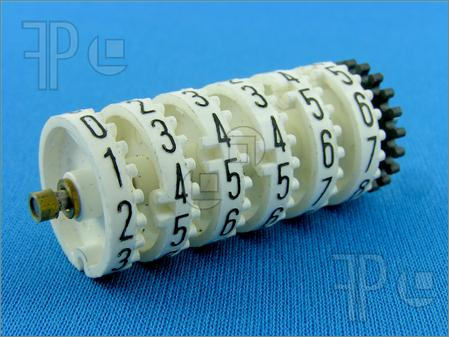
\includegraphics[scale=0.66]{modulo/counter.jpg}
\caption{The picture was stolen from \url{http://www.featurepics.com/} --- sorry for that!}
\end{figure}

This counter has 6 wheels, so it can count from 0 to $10^{6}-1$ or 999999.
When you have 999999 and you increase the counter, it will resetting to 000000---
this situation is usually understood by engineers and computer programmers as overflow.
And if you have 000000 and you decrease it, the counter will show you 999999.
This situation is often called ``wrap around''.
See also: \url{http://en.wikipedia.org/wiki/Integer_overflow}.

\myheading{Modular arithmetic on CPUs}

The reason I talk about mechanical counter is that CPU registers acting in the very same way, because this is, perhaps, simplest possible and efficient way
to compute using integer numbers.

This implies that almost all operations on integer values on your CPU is happens by modulo $2^{32}$ or $2^{64}$ depending on your CPU.
For example, you can sum up 0x87654321 and 0xDEADBABA, which resulting in 0x16612FDDB.
This value is too big for 32-bit register, so only 0x6612FDDB is stored, and leading 1 is dropped.
If you will multiply these two numbers, the actual result it 0x75C5B266EDA5BFFA, which is also too big, so only low 32-bit part is stored into destination
register: 0xEDA5BFFA. This is what happens when you multiply numbers in plain C/C++ language, but some readers may argue:
when sum is too big for register, CF (carry flag) is set, and it can be used after.
And there is x86 MUL instruction which in fact produces 64-bit result in 32-bit environment (in EDX:EAX registers pair).
That's true, but observing just 32-bit registers, this is exactly environment of modulo with base $2^{32}$.

Now that leads to surprising consequence: almost every result of arithmetic operation stored in general purpose register of
32-bit CPU is in fact
remainder of division operation: result is always divided by $2^{32}$ and remainder is left in register.
For example, 0x16612FDDB is too large for storage, and it's divided by $2^{32}$ (or 0x100000000).
The result of division (quotient) is 1 (which is dropped) and remainder is 0x6612FDDB (which is stored as a result).
0x75C5B266EDA5BFFA divided by $2^{32}$ (0x100000000) produces 0x75C5B266 as a result of division (quotient) and 0xEDA5BFFA as a remainder, the latter is stored.

And if your code is 32-bit one in 64-bit environment, CPU registers are bigger, so the whole result can be stored there,
but high half is hidden behind the scenes -- because no 32-bit code can access it.

By the way, this is the reason why remainder calculation is often called "division by modulo".
C/C++ has a percent sign (``\%'') for this operation, but some other PLs like Pascal and Haskell has "mod" operator.

Usually, almost all sane computer programmers works with variables as they never wrapping around and value here is always in some limits which
are defined preliminarily.
However, this implicit division operation or "wrapping around" can be exploited usefully.

\myheading{Remainder of division by modulo $2^{n}$}

... can be easily computed with AND operation.
If you need a random number in range of 0..16, here you go: rand()\&0xF.
That helps sometimes.</p>

<p>For example, you need a some kind of wrapping counter variable which always should be in 0..16 range. What you do?
Programmers often write this:

\begin{lstlisting}[style=customc]
int counter=0;
...
counter++;
if (counter==16)
    counter=0;
\end{lstlisting}

But here is a version without conditional branching:

\begin{lstlisting}[style=customc]
int counter=0;
...
counter++;
counter=counter&0xF;
\end{lstlisting}

As an example, this I found in the git source code:

\begin{lstlisting}[style=customc]
char *sha1_to_hex(const unsigned char *sha1)
{
        static int bufno;
        static char hexbuffer[4][GIT_SHA1_HEXSZ + 1];
        static const char hex[] = "0123456789abcdef";
        char *buffer = hexbuffer[3 & ++bufno], *buf = buffer;
        int i;

        for (i = 0; i < GIT_SHA1_RAWSZ; i++) {
                unsigned int val = *sha1++;
                *buf++ = hex[val >> 4];
                *buf++ = hex[val & 0xf];
        }
        *buf = '\0';

        return buffer;
}
\end{lstlisting}

( \url{https://github.com/git/git/blob/aa1c6fdf478c023180e5ca5f1658b00a72592dc6/hex.c} )

This function returns a pointer to the string containing hexadecimal representation of SHA1 digest \\
(like "4e1243bd22c66e76c2ba9eddc1f91394e57f9f83").
But this is plain C and you can calculate SHA1 for some block, get pointer to the string, then calculate SHA1 for another block, get pointer to the string,
and both pointers are still points to the same string buffer containing the result of the second calculation.
As a solution, it's possible to allocate/deallocate string buffer each time, but more hackish way is to have several buffers (4 are here) and fill the next each time.
The \textit{bufno} variable here is a buffer counter in 0..3 range.
Its value increments each time, and its value is also always
kept in limits
by AND operation (\textit{3 \& ++bufno}).

The author of this piece of code (seemingly Linus Torvalds himself) went even further and forgot (?)
to initialize \textit{bufno} counter variable, which will
have random garbage at the function start.
Indeed: no matter, which buffer we are starting each time!
This can be mistake which isn't affect correctness of the code, or maybe this is left so intentionally -- I don't know.

\myheading{Getting random numbers}

When you write some kind of videogame, you need random numbers, and the standard C/C++ rand() function gives you them in 0..0x7FFF range (MSVC)
or in 0..0x7FFFFFFF range (GCC).
And when you need a random number in 0..10 range, the common way to do it is:

\begin{lstlisting}
X_coord_of_something_spawned_somewhere=rand() % 10;
Y_coord_of_something_spawned_somewhere=rand() % 10;
\end{lstlisting}

No matter what compiler do you use, you can think about it as 10 is subtraced from rand() result, as long as there is still
a number bigger than 10.
Hence, result is remainder of division of rand() result by 10.

One nasty consequence is that neither 0x8000 nor 0x80000000 cannot be divided by 10 evenly, so you'll get some numbers slightly more often than others.

I tried to calculate in Mathematica. Here is what you get if you write <i>rand() % 3</i> and rand() produce numbers in range of 0..0x7FFF (like MSVC):

\begin{lstlisting}
In[]:= Counts[Map[Mod[#, 3] &, Range[0, 16^^8000 - 1]]]
Out[]= <|0 -> 10923, 1 -> 10923, 2 -> 10922|>
\end{lstlisting}

So a number 2 appers slightly seldom than others.

Here is a result for \textit{rand() \% 10}:

\begin{lstlisting}
In[]:= Counts[Map[Mod[#, 10] &, Range[0, 16^^8000 - 1]]]
Out[]= <|0 -> 3277, 1 -> 3277, 2 -> 3277, 3 -> 3277, 4 -> 3277,
 5 -> 3277, 6 -> 3277, 7 -> 3277, 8 -> 3276, 9 -> 3276|>
\end{lstlisting}

Numbers 8 and 9 appears slightly seldom.

Here is a result for \textit{rand() \% 100}:

\begin{lstlisting}
In[]:= Counts[Map[Mod[#, 100] &, Range[0, 16^^8000 - 1]]]
Out[]= <|0 -> 328, 1 -> 328, 2 -> 328, 3 -> 328, 4 -> 328, 5 -> 328,
  6 -> 328, 7 -> 328, 8 -> 328, 9 -> 328, 10 -> 328, 11 -> 328,
 12 -> 328, 13 -> 328, 14 -> 328, 15 -> 328, 16 -> 328, 17 -> 328,
 18 -> 328, 19 -> 328, 20 -> 328, 21 -> 328, 22 -> 328, 23 -> 328,
 24 -> 328, 25 -> 328, 26 -> 328, 27 -> 328, 28 -> 328, 29 -> 328,
 30 -> 328, 31 -> 328, 32 -> 328, 33 -> 328, 34 -> 328, 35 -> 328,
 36 -> 328, 37 -> 328, 38 -> 328, 39 -> 328, 40 -> 328, 41 -> 328,
 42 -> 328, 43 -> 328, 44 -> 328, 45 -> 328, 46 -> 328, 47 -> 328,
 48 -> 328, 49 -> 328, 50 -> 328, 51 -> 328, 52 -> 328, 53 -> 328,
 54 -> 328, 55 -> 328, 56 -> 328, 57 -> 328, 58 -> 328, 59 -> 328,
 60 -> 328, 61 -> 328, 62 -> 328, 63 -> 328, 64 -> 328, 65 -> 328,
 66 -> 328, 67 -> 328, 68 -> 327, 69 -> 327, 70 -> 327, 71 -> 327,
 72 -> 327, 73 -> 327, 74 -> 327, 75 -> 327, 76 -> 327, 77 -> 327,
 78 -> 327, 79 -> 327, 80 -> 327, 81 -> 327, 82 -> 327, 83 -> 327,
 84 -> 327, 85 -> 327, 86 -> 327, 87 -> 327, 88 -> 327, 89 -> 327,
 90 -> 327, 91 -> 327, 92 -> 327, 93 -> 327, 94 -> 327, 95 -> 327,
 96 -> 327, 97 -> 327, 98 -> 327, 99 -> 327|>
\end{lstlisting}

\dots now larger part of numbers happens slightly seldom, these are 68...99.

This is sometimes called \textit{modulo bias}. It's perhaps acceptable for videogames, but may be critical for scientific simulations, including Monte Carlo method.

Constructing a \ac{PRNG} with uniform distribution may be tricky, there are couple of methods:
\url{http://www.reddit.com/r/algorithms/comments/39tire/using_a_01_generator_generate_a_random_number/},
\url{http://www.prismmodelchecker.org/casestudies/dice.php}.

\levelup{}


\myheading{Modulo inverse}

Example: this piece of code divides by 17:

\begin{lstlisting}[style=customc]
#include <stdio.h>
#include <stdint.h>

uint32_t div17 (uint32_t a)
{
	return a*0xf0f0f0f1;
};

int main()
{
	printf ("%d\n", div17(1700));	// result=100
	printf ("%d\n", div17(34));	// result=2
	printf ("%d\n", div17(2091));	// result=123
};
\end{lstlisting}

Unfortunately, it can't produce correct quotient if $remainder \neq 0$, so it's not very useful.
But this code (which divides by 9, though) works correctly in all cases:

\begin{lstlisting}[style=customc]
#include <stdint.h>

uint32_t divide_by_9 (uint32_t a)
{
        return ((uint64_t)a * (uint64_t)954437177) >> 33; // 954437177 = 0x38e38e39
};
\end{lstlisting}

How it works?

\myhrule{}

Let's imagine, we work on 4-bit CPU, it has 4-bit registers, each can hold a value in 0..15 range.

Now we want to divide by 3 using multiplication.
Let's find modulo inverse of 3 using Wolfram Mathematica:

\begin{lstlisting}
In[]:= PowerMod[3, -1, 16]
Out[]= 11
\end{lstlisting}

This is in fact solution of a $3m=16k+1$ equation ($16 = 2^4$):

\begin{lstlisting}
In[]:= FindInstance[3 m == 16 k + 1, {m, k}, Integers]
Out[]= {{m -> 11, k -> 2}}
\end{lstlisting}

The "magic number" for division by 3 is 11. Multiply by 11 instead of dividing by 3 and you'll get a result (quotient).

This works, let's divide 6 by 3. We can now do this by multiplying 6 by 11, this is 66=0x42,
but on 4-bit register, only 0x2 will be left in register ($0x42 \equiv 2 \mod 2^4$).
Yes, 2 is correct answer, 6/3=2.

Let's divide 3, 6 and 9 by 3, by multiplying by 11 (m).

\iffalse
% FIXME: texify
\begin{lstlisting}[basicstyle=\tiny]
           |123456789abcdef0|123456789abcdef0|123456789abcdef0|123456789abcdef0|123456789abcdef0|123456789abcdef0|123456789abcdef0|
    m=11   |***********     |                |                |                |                |                |                |
3/3 3m=33  |****************|****************|*               |                |                |                |                |
6/3 6m=66  |****************|****************|****************|****************|**              |                |                |
9/3 9m=99  |****************|****************|****************|****************|****************|****************|***             |
\end{lstlisting}
\fi

%\begin{lstlisting}[basicstyle=\small]
\begin{lstlisting}[basicstyle=\footnotesize]
           |123456789abcdef0|12 ... f0|123456789abcdef0|12 ... f0|123456789abcdef0|12 ... f0|123456789abcdef0|
    m=11   |***********     |   ...   |                |   ...   |                |   ...   |                |
3/3 3m=33  |****************|** ... **|*               |   ...   |                |   ...   |                |
6/3 6m=66  |****************|** ... **|****************|** ... **|**              |   ...   |                |
9/3 9m=99  |****************|** ... **|****************|** ... **|****************|** ... **|***             |
\end{lstlisting}

A "protruding" asterisk(s) (*) in the last non-empty chunk is what will be left in 4-bit register.
This is 1 in case of 33, 2 if 66, 3 if 99.

In fact, this "protrusion" is defined by 1 in the equation we've solved.
Let's replace 1 with 2:

\begin{lstlisting}
In[]:= FindInstance[3 m == 16 k + 2, {m, k}, Integers]
Out[]= {{m -> 6, k -> 1}}
\end{lstlisting}

Now the new "magic number" is 6.
Let's divide 3 by 3. 3*6=18=0x12, 2 will be left in 4-bit register. This is incorrect, we have 2 instead of 1. 2 asterisks are "protruding".
Let's divide 6 by 3. 6*6=36=0x24, 4 will be left in the register. This is also incorrect, we now have 4 "protruding" asterisks instead of correct 2.

Replace 1 in the equation by 0, and nothing will "protrude".

Now the problem: this only works for dividends in 3x form, i.e., which can be divided by 3 with no remainder.
Try to divide 4 by 3, 4*11=44=0x2c, 12 will be left in register, this is incorrect.
The correct quotient is 1.

We can also notice that the 4-bit register is "overflown" during multiplication twice as much as in "incorrect" result in low 4 bits.

Here is what we can do: use only high 4 bits and drop low 4 bits.
4*11=0x2c and 2 is high 4 bits.
Divide 2 by 2, this is 1.

Let's "divide" 8 by 3. 8*11=88=0x58. 5/2=2, this is correct answer again.

Now this is the formula we can use on our 4-bit CPU to divide numbers by 3: "x*3 >> 4 / 2" or "x*3 >> 5".
This is the same as almost all modern compilers do instead of integer division, but they do this for 32-bit and 64-bit registers.


\myheading{Reversible linear congruential generator}

\ac{LCG} \ac{PRNG} is very simple: just multiply seed by some value, add another one and here is a new random number.
Here is how it is implemented in MSVC (the source code is not original one and is reconstructed by me):</p>

\begin{lstlisting}[style=customc]
uint32_t state;

uint32_t rand()
{
	state=state*214013+2531011;
	return (state>>16)&0x7FFF;
};
\end{lstlisting}

The last bit shift is attempt to compensate LCG weakness and we may ignore it so far.
Will it be possible to make an inverse function to rand(), which can reverse state back?
First, let's try to think, what would make this possible? Well, if state internal variable would be some kind of BigInt or BigNum container which can
store infinitely big numbers, then, although state is increasing rapidly, it would be possible to reverse the process.
But \textit{state} isn't BigInt/BigNum, it's 32-bit variable, and summing operation is easily reversible on it (just subtract 2531011 at each step).
As we may know now, multiplication is also reversible: just multiply the state by modular multiplicative inverse of 214013!

\begin{lstlisting}[style=customc]
#include <stdio.h>
#include <stdint.h>

uint32_t state;

void next_state()
{
	state=state*214013+2531011;
};

void prev_state()
{
	state=state-2531011; // reverse summing operation
	state=state*3115528533; // reverse multiply operation. 3115528533 is modular inverse of 214013 in $2^{32}$.
};

int main()[style=customc]
{
	state=12345;
	
	printf ("state=%d\n", state);
	next_state();
	printf ("state=%d\n", state);
	next_state();
	printf ("state=%d\n", state);
	next_state();
	printf ("state=%d\n", state);

	prev_state();
	printf ("state=%d\n", state);
	prev_state();
	printf ("state=%d\n", state);
	prev_state();
	printf ("state=%d\n", state);
};
\end{lstlisting}

Wow, that works!

\begin{lstlisting}
state=12345
state=-1650445800
state=1255958651
state=-456978094
state=1255958651
state=-1650445800
state=12345
\end{lstlisting}

It's hard to find a real-world application of reversible LCG, but this could be the one:
a media player with forward/backward buttons.
Once shuffle is clicked, random number is generated (number of item to be played).
User clicks forward: get a new random number by calculating the next state.
User clicks backward: get it by calculating the previous state.
Thus, a user could navigate through some "virtual" (but consistent) playlist, which is even not present in media player's memory!



\levelup{}


\newchapter{Probability}

\leveldown{}

\myheading{Text strings right in the middle of compressed data}

%\myindex{Linux kernel}
You can download Linux kernels and find English words right in the middle of compressed data:

\begin{lstlisting}
% wget https://www.kernel.org/pub/linux/kernel/v4.x/linux-4.10.2.tar.gz

% xxd -g 1 -seek 0x515c550 -l 0x30 linux-4.10.2.tar.gz

0515c550: c5 59 43 cf 41 27 85 54 35 4a 57 90 73 89 b7 6a  .YC.A'.T5JW.s..j
0515c560: 15 af 03 db 20 df 6a 51 f9 56 49 52 55 53 3d da  .... .jQ.VIRUS=.
0515c570: 0e b9 29 24 cc 6a 38 e2 78 66 09 33 72 aa 88 df  ..)$.j8.xf.3r...
\end{lstlisting}

\begin{lstlisting}
% wget https://cdn.kernel.org/pub/linux/kernel/v2.3/linux-2.3.3.tar.bz2

% xxd -g 1 -seek 0xa93086 -l 0x30 linux-2.3.3.tar.bz2

00a93086: 4d 45 54 41 4c cd 44 45 2d 2c 41 41 54 94 8b a1  METAL.DE-,AAT...
00a93096: 5d 2b d8 d0 bd d8 06 91 74 ab 41 a0 0a 8a 94 68  ]+......t.A....h
00a930a6: 66 56 86 81 68 0d 0e 25 6b b6 80 a4 28 1a 00 a4  fV..h..%k...(...
\end{lstlisting}

One of Linux kernel patches in compressed form has the ``Linux'' word itself:

\begin{lstlisting}
% wget https://cdn.kernel.org/pub/linux/kernel/v4.x/testing/patch-4.6-rc4.gz

% xxd -g 1 -seek 0x4d03f -l 0x30 patch-4.6-rc4.gz

0004d03f: c7 40 24 bd ae ef ee 03 2c 95 dc 65 eb 31 d3 f1  .@$.....,..e.1..
0004d04f: 4c 69 6e 75 78 f2 f3 70 3c 3a bd 3e bd f8 59 7e  Linux..p<:.>..Y~
0004d05f: cd 76 55 74 2b cb d5 af 7a 35 56 d7 5e 07 5a 67  .vUt+...z5V.^.Zg
\end{lstlisting}

Other English words I've found in other compressed Linux kernel trees:

\begin{lstlisting}
linux-4.6.2.tar.gz: [maybe] at 0x68e78ec
linux-4.10.14.tar.xz: [OCEAN] at 0x6bf0a8
linux-4.7.8.tar.gz: [FUNNY] at 0x29e6e20
linux-4.6.4.tar.gz: [DRINK] at 0x68dc314
linux-2.6.11.8.tar.bz2: [LUCKY] at 0x1ab5be7
linux-3.0.68.tar.gz: [BOOST] at 0x11238c7
linux-3.0.16.tar.bz2: [APPLE] at 0x34c091
linux-3.0.26.tar.xz: [magic] at 0x296f7d9
linux-3.11.8.tar.bz2: [TRUTH] at 0xf635ba
linux-3.10.11.tar.bz2: [logic] at 0x4a7f794
\end{lstlisting}

%\myindex{Apophenia}
%\myindex{Pareidolia}
%\myindex{Lurkmore}
There is a nice illustration of apophenia and pareidolia
(human's mind ability to see faces in clouds, etc) in Lurkmore, Russian counterpart of Encyclopedia Dramatica.
As they wrote in the article about electronic voice phenomenon\footnote{\url{http://archive.is/gYnFL}},
you can open any long enough compressed file in hex editor and find well-known 3-letter Russian obscene word, and you'll find it a lot: but that means nothing, just a mere coincidence.

And I was interested in calculation, how big compressed file must be to contain all possible 3-letter, 4-letter, etc, words?
In my naive calculations, I've got this: probability of the first specific byte in the middle of compressed data stream with maximal entropy is $\frac{1}{256}$, probability of the 2nd is also $\frac{1}{256}$,
and probability of specific byte pair is $\frac{1}{256 \cdot 256} = \frac{1}{256^2}$.
Probabilty of specific triple is $\frac{1}{256^3}$.
If the file has maximal entropy (which is almost unachievable, but \dots) and we live in an ideal world, you've got to have a file of size just $256^3=16777216$, which is 16-17MB.
%\myindex{rafind2}
You can check: get any compressed file, and use \textit{rafind2} to search for any 3-letter word (not just that Russian obscene one).

It took $\approx$ 8-9 GB of my downloaded movies/TV series files to find the word ``beer'' in them (case sensitive).
Perhaps, these movies wasn't compressed good enough?
This is also true for a well-known 4-letter English obscene word.

My approach is naive, so I googled for mathematically grounded one, and have find this question:
``Time until a consecutive sequence of ones in a random bit sequence''
\footnote{\url{http://math.stackexchange.com/questions/27989/time-until-a-consecutive-sequence-of-ones-in-a-random-bit-sequence/27991\#27991}}.
The answer is: $(p^{−n}−1)/(1−p)$, where $p$ is probability of each event and $n$ is number of consecutive events.
Plug $\frac{1}{256}$ and $3$ and you'll get almost the same as my naive calculations.

So any 3-letter word can be found in the compressed file (with ideal entropy) of length $256^3 = \approx 17MB$, any 4-letter word --- $256^4 = 4.7GB$ (size of DVD).
Any 5-letter word --- $256^5 = \approx 1TB$.

For the piece of text you are reading now, I mirrored the whole \href{https://www.kernel.org/}{kernel.org} website (hopefully, sysadmins can forgive me),
and it has $\approx$ 430GB of compressed Linux Kernel source trees.
It has enough compressed data to contain these words, however, I cheated a bit: I searched for both lowercase and uppercase strings, thus compressed data set I need is almost halved.

This is quite interesting thing to think about: 1TB of compressed data with maximal entropy has all possible 5-byte chains,
but the data is encoded not in chains itself, but in the order of chains (no matter of compression algorithm, etc).

Now the information for gamblers: one should throw a dice $\approx 42$ times to get a pair of six, but no one will tell you, when exactly this will happen.
%\myindex{Rosencrantz \& Guildenstern Are Dead}
I don't remember, how many times coin was tossed in the ``Rosencrantz \& Guildenstern Are Dead'' movie, but one should toss it $\approx 2048$ times and at some point, you'll get 10 heads in a row,
and at some other point, 10 tails in a row. Again, no one will tell you, when exactly this will happen.

Compressed data can also be treated as a stream of random data, so we can use the same mathematics to determine probabilities, etc.

If you can live with strings of mixed case, like ``bEeR'', probabilities and compressed data sets are much lower:
$128^3=2MB$ for all 3-letter words of mixed case,
$128^4=268MB$ for all 4-letter words,
$128^5=34GB$ for all 5-letter words, etc.

%\myindex{Jorge Luis Borges}
Moral of the story: whenever you search for some patterns, you can find it in the middle of compressed blob, but that means nothing else then coincidence.
In philosophical sense, this is a case of selection/confirmation bias: you find what you search for in ``The Library of Babel''\footnote{Short story by Jorge Luis Borges}.



\levelup{}


\myheading{Combinatorics}

\leveldown{}

\myheading{Soldering a headphones cable}

Let's say, a cable have 3 wires, red/green/blue.
Which is left/right and ground?
Let's say, you can try all possible combinations.

All permutations of 3 wires is 3!=6.

\begin{lstlisting}[caption=Wolfram Mathematica]
In[]:= Permutations[{red, green, blue}]

Out[]= {{red, green, blue}, {red, blue, green}, {green, red, blue}, {green, blue, red}, {blue, red, green}, {blue, green, red}}
\end{lstlisting}

What if 4 wires?

4!=24.

\begin{lstlisting}[caption=Wolfram Mathematica]
In[]:= Permutations[{red, green, blue , yellow}]

Out[]= {{red, green, blue, yellow}, {red, green, yellow, blue}, {red, blue, green, yellow}, {red, blue, yellow, green}, {red, yellow, green, blue}, {red, yellow, blue, green}, {green, red, blue, yellow}, {green, red, yellow, blue}, {green, blue, red, yellow}, {green, blue, yellow, red}, {green, yellow, red, blue}, {green, yellow, blue, red}, {blue, red, green, yellow}, {blue, red, yellow, green}, {blue, green, red, yellow}, {blue, green, yellow, red}, {blue, yellow, red, green}, {blue, yellow, green, red}, {yellow, red, green, blue}, {yellow, red, blue, green}, {yellow, green, red, blue}, {yellow, green, blue, red}, {yellow, blue, red, green}, {yellow, blue, green, red}}
\end{lstlisting}


\myheading{Executable file watermarking/steganography using Lehmer code and factorial number system}

In short: how to hide information not in objects, but in \textit{order} of objects.

Almost any binary executable file has text strings like (these are from CRT):

\begin{lstlisting}
.rdata:0040D398 aR6002FloatingP:
.rdata:0040D398                 text "UTF-16LE", 'R6002',0Dh,0Ah
.rdata:0040D398                 text "UTF-16LE", '- floating point support not loaded',0Dh,0Ah,0
.rdata:0040D3F2                 align 8
.rdata:0040D3F8 aR6008NotEnough:
.rdata:0040D3F8                 text "UTF-16LE", 'R6008',0Dh,0Ah
.rdata:0040D3F8                 text "UTF-16LE", '- not enough space for arguments',0Dh,0Ah,0
.rdata:0040D44C                 align 10h
.rdata:0040D450 aR6009NotEnough:
.rdata:0040D450                 text "UTF-16LE", 'R6009',0Dh,0Ah
.rdata:0040D450                 text "UTF-16LE", '- not enough space for environment',0Dh,0Ah,0
.rdata:0040D4A8 aR6010AbortHasB:
.rdata:0040D4A8                 text "UTF-16LE", 'R6010',0Dh,0Ah
.rdata:0040D4A8                 text "UTF-16LE", '- abort() has been called',0Dh,0Ah,0
.rdata:0040D4EE                 align 10h
.rdata:0040D4F0 aR6016NotEnough:
.rdata:0040D4F0                 text "UTF-16LE", 'R6016',0Dh,0Ah
.rdata:0040D4F0                 text "UTF-16LE", '- not enough space for thread data',0Dh,0Ah,0
.rdata:0040D548 aR6017Unexpecte:
.rdata:0040D548                 text "UTF-16LE", 'R6017',0Dh,0Ah
.rdata:0040D548                 text "UTF-16LE", '- unexpected multithread lock error',0Dh,0Ah,0
.rdata:0040D5A2                 align 8
.rdata:0040D5A8 aR6018Unexpecte:
.rdata:0040D5A8                 text "UTF-16LE", 'R6018',0Dh,0Ah
.rdata:0040D5A8                 text "UTF-16LE", '- unexpected heap error',0Dh,0Ah,0
.rdata:0040D5EA                 align 10h
\end{lstlisting}

Can we hide some information there?
Not in string themselves, but in \textit{order} of strings?
Given the fact, that compiler doesn't guarantee at all,
in which order the strings will be stored in object/executable file.

Let's say, we've got 26 text strings, and we can swap them how we want, because their order isn't important at all.
All possible permutations of 26 objects is 
26! = 403291461126605635584000000.

How much information can be stored here?
log2(26!)=~88, i.e., 88 bits or 11 bytes!

11 bytes of your data can be converted to a (big) number and back, OK.

What is next?
Naive way is: enumerate all permutations of 26 objects, number each, find permutation of the number we've got and
permute 26 text strings, store to file and that's it.
But we can't iterate over 403291461126605635584000000 permutations.

This is where factorial number system
\footnote{\url{https://en.wikipedia.org/wiki/Factorial_number_system}}
and Lehmer code
\footnote{\url{https://en.wikipedia.org/wiki/Lehmer_code}}
can be used.
In short, for all my non-mathematically inclined readers, this is a way to find a permutation of specific number
without use of any significant resources.
And back: gived specific permutation, we can find its number.

This piece of code I've copypasted from \url{https://gist.github.com/lukmdo/7049748} and reworked slightly:

\lstinputlisting[style=custompy]{comb/lehmer/lehmer.py}

I'm encoding a "HelloWorld" binary string (in fact, any 11 bytes can be used) into a number.
Number is then converted into Lehmer code.
Then the perm\_from\_code() function permute initial \textit{order} according to the input Lehmer code:

\begin{lstlisting}
s= HelloWorld
num= 341881320659934023674980
Lehmer code= [14, 16, 7, 16, 7, 11, 17, 7, 1, 4, 10, 7, 9, 11, 6, 2, 6, 1, 2, 4, 0, 0, 0, 0, 0, 0]
swapping 0, 14
swapping 1, 17
swapping 2, 9
swapping 3, 19
swapping 4, 11
swapping 5, 16
swapping 6, 23
swapping 7, 14
swapping 8, 9
swapping 9, 13
swapping 10, 20
swapping 11, 18
swapping 12, 21
swapping 13, 24
swapping 14, 20
swapping 15, 17
swapping 16, 22
swapping 17, 18
swapping 18, 20
swapping 19, 23
permutation/order= [14, 17, 9, 19, 11, 16, 23, 0, 2, 13, 20, 18, 21, 24, 10, 1, 22, 4, 7, 6, 15, 12, 5, 3, 8, 25]
\end{lstlisting}

This is it: [14, 17, 9, 19, 11, 16, 23, 0, 2, 13, 20, 18, 21, 24, 10, 1, 22, 4, 7, 6, 15, 12, 5, 3, 8, 25].
First put 14th string, then 17s string, then 9th one, etc.

Now you've got a binary file from someone and want to read watermark from it.
Get an order of strings from it and convert it back to binary string:

\begin{lstlisting}
recovered num= 341881320659934023674980
recovered s= HelloWorld
\end{lstlisting}

If you have more text strings (not unusual for most executable files), you can encode more.

100 strings: log2(100!) = ~524 bits = ~65 bytes.

1000 strings: log2(1000!) = ~8529 bits = ~1066 bytes! You can store some text here!

How would you force a C/C++ compiler to make specific order of text strings?
This is crude, but workable:

\begin{lstlisting}
char blob[]="hello1\0hello2\0";
char *msg1=blob;
char *msg2=blob+8;

printf ("%s\n", msg1);
printf ("%s\n", msg2);
\end{lstlisting}

They can be even aligned on 16-byte border.

... or they can be placed into .s/.asm assembly file and compiled into .o/.obj and then linked to your program.

... or you can swap text strings in already compiled executable and correct their addresses in corresponding instructions.
If an executable file is not packed/obfuscated, this is possible.

Aside of order of text strings, you can try to hack a linker and reorder object files in the final executable.
Of course, no one cares about its order.
And go figure out, what is hidden there.

Surely, hidden data can be encrypted, checksum or MAC can be added, etc.

Other ideas to consider: reorder functions and fix all addresses,
reorder basic blocks within a function, register allocator hacking, etc.

Links I find helpful in understanding factorial number system and Lehmer code, aside of Wikipedia:

\begin{itemize}
\item \url{https://gist.github.com/lukmdo/7049748}
\item \url{https://github.com/scmorse/permutils/blob/master/src/permutils.js}
\item \url{http://2ality.com/2013/03/permutations.html}
\item \url{http://www.keithschwarz.com/interesting/code/factoradic-permutation/FactoradicPermutation}
\end{itemize}


\myheading{De Bruijn sequences; leading/trailing zero bits counting}

\leveldown{}

\myheading{Introduction}

Let's imagine there is a very simplified code lock accepting 2 digits, but it has no "enter" key, it just checks 2 last entered digits.
Our task is to brute force each 2-digit combination.
Naïve method is to try 00, 01, 02 ... 99.
That require 2*100=200 key pressings.
Will it be possible to reduce number of key pressings during brute-force?
It is indeed so, with the help of De Bruijn sequences.
We can generate them for the code lock, using Wolfram Mathematica:

\begin{lstlisting}
In[]:= DeBruijnSequence[{0, 1, 2, 3, 4, 5, 6, 7, 8, 9}, 2]
Out[]= {6, 8, 6, 5, 4, 3, 2, 1, 7, 8, 7, 1, 1, 0, 9, 0, 8, 0, 6, 6, \
0, 5, 5, 0, 4, 4, 0, 3, 3, 0, 2, 7, 2, 2, 0, 7, 7, 9, 8, 8, 9, 9, 7, \
0, 0, 1, 9, 1, 8, 1, 6, 1, 5, 1, 4, 1, 3, 7, 3, 1, 2, 9, 2, 8, 2, 6, \
2, 5, 2, 4, 7, 4, 2, 3, 9, 3, 8, 3, 6, 3, 5, 7, 5, 3, 4, 9, 4, 8, 4, \
6, 7, 6, 4, 5, 9, 5, 8, 5, 6, 9}
\end{lstlisting}

The result has exactly 100 digits, which is 2 times less than our initial idea can offer.
By scanning visually this 100-digits array, you'll find any number in 00..99 range.
All numbers are overlapped with each other: second half of each number is also first half of the next number, etc.

Here is another. We need a sequence of binary bits with all 3-bit numbers in it:

\begin{lstlisting}
In[]:= DeBruijnSequence[{0, 1}, 3]
Out[]= {1, 0, 1, 0, 0, 0, 1, 1}
\end{lstlisting}

Sequence length is just 8 bits, but it has all binary numbers in 000..111 range.
You may visually spot 000 in the middle of sequence.
111 is also present: two first bits of it at the end of sequence and the last bit is in the beginning.
This is so because De Bruijn sequences are cyclic.

There is also visual demonstration: \url{http://demonstrations.wolfram.com/DeBruijnSequences/}.

\myheading{Trailing zero bits counting}

In \href{https://en.wikipedia.org/wiki/De_Bruijn_sequence}{the Wikipedia article about De Bruijn sequences} we can find:

\begin{framed}
\begin{quotation}
The symbols of a De Bruijn sequence written around a circular object (such as a wheel of a robot) can be used to identify its angle by examining the n consecutive symbols facing a fixed point.
\end{quotation}
\end{framed}

Indeed: if we know De Bruijn sequence and we observe only part of it (any part), we can deduce exact position of this part within sequence.

Let's see, how this feature can be used.

Let's say, there is a need to detect position of input bit within 32-bit word.
For 0x1, the algorithm should report 1.
2 for 0x2.
3 for 0x4.
And 31 for 0x80000000.

The result is in 0..31 range, so the result can be stored in 5 bits.

We can construct binary De Bruijn sequence for all 5-bit numbers:

\begin{lstlisting}
In[]:= tmp = DeBruijnSequence[{0, 1}, 5]
Out[]= {1, 1, 1, 0, 0, 1, 1, 0, 1, 0, 1, 1, 1, 1, 1, 0, 1, 1, 0, 0, 0, 1, 0, 1, 0, 0, 1, 0, 0, 0, 0, 0}

In[]:= BaseForm[FromDigits[tmp, 2], 16]
Out[]:= e6bec520
\end{lstlisting}

Let's also recall that division some number by $2^n$ number is the same thing as shifting it by $n$ bits.
So if you divide 0xe6bec520 by 1, the result is not shifted, it is still the same.
If if divide 0xe6bec520 by 4 ($2^2$), the result is shifted by 2 bits.
We then take result and isolate lowest 5 bits.
This result is unique number for each input.
Let's shift 0xe6bec520 by all possible count number, and we'll get all possible last 5-bit values:

\begin{lstlisting}
In[]:= Table[BitAnd[BitShiftRight[FromDigits[tmp, 2], i], 31], {i, 0, 31}]
Out[]= {0, 16, 8, 4, 18, 9, 20, 10, 5, 2, 17, 24, 12, 22, 27, 29, \
30, 31, 15, 23, 11, 21, 26, 13, 6, 19, 25, 28, 14, 7, 3, 1}
\end{lstlisting}

The table has no duplicates:

\begin{lstlisting}
In[]:= DuplicateFreeQ[%]
Out[]= True
\end{lstlisting}

Using this table, it's easy to build a \textit{magic} table.
OK, now working C example:

\begin{lstlisting}[style=customc]
#include <stdint.h>
#include <stdio.h>

int magic_tbl[32];

// returns single bit position counting from LSB
// not working for i==0
int bitpos (uint32_t i)
{
	return magic_tbl[(0xe6bec520/i) & 0x1F];
};

int main()
{
	// construct magic table
	// may be omitted in production code
	for (int i=0; i<32; i++)
		magic_tbl[(0xe6bec520/(1<<i)) & 0x1F]=i;

	// test
	for (int i=0; i<32; i++)
	{
		printf ("input=0x%x, result=%d\n", 1<<i, bitpos (1<<i));
	};
};
\end{lstlisting}

Here we feed our bitpos() function with numbers in 0..0x80000000 range and we got:

\begin{lstlisting}
input=0x1, result=0
input=0x2, result=1
input=0x4, result=2
input=0x8, result=3
input=0x10, result=4
input=0x20, result=5
input=0x40, result=6
input=0x80, result=7
input=0x100, result=8
input=0x200, result=9
input=0x400, result=10
input=0x800, result=11
input=0x1000, result=12
input=0x2000, result=13
input=0x4000, result=14
input=0x8000, result=15
input=0x10000, result=16
input=0x20000, result=17
input=0x40000, result=18
input=0x80000, result=19
input=0x100000, result=20
input=0x200000, result=21
input=0x400000, result=22
input=0x800000, result=23
input=0x1000000, result=24
input=0x2000000, result=25
input=0x4000000, result=26
input=0x8000000, result=27
input=0x10000000, result=28
input=0x20000000, result=29
input=0x40000000, result=30
input=0x80000000, result=31
\end{lstlisting}

The bitpos() function actually counts trailing zero bits, but it works only for input values where only one bit is set.
To make it more practical, we need to devise a method to drop all leading bits except of the last one.
This method is very simple and well-known:

\begin{lstlisting}
input & (-input)
\end{lstlisting}

This bit twiddling hack can solve the job. Feeding 0x11 to it, it will return 0x1. Feeding 0xFFFF0000, it will return 0x10000.
In other words, it leaves lowest significant bit of the value, dropping all others.

It works because negated value in two's complement environment is the value with all bits flipped but also 1 added (because there is a zero in the middle of ring).
For example, let's take 0xF0. -0xF0 is 0x10 or 0xFFFFFF10. ANDing 0xF0 and 0xFFFFFF10 will produce 0x10.

Let's modify our algorithm to support true trailing zero bits count:

\begin{lstlisting}[style=customc]
#include <stdint.h>
#include <stdio.h>

int magic_tbl[32];

// not working for i==0
int tzcnt (uint32_t i)
{
	uint32_t a=i & (-i);
	return magic_tbl[(0xe6bec520/a) & 0x1F];
};

int main()
{
	// construct magic table
	// may be omitted in production code
	for (int i=0; i<32; i++)
		magic_tbl[(0xe6bec520/(1<<i)) & 0x1F]=i;

	// test:
	printf ("%d\n", tzcnt (0xFFFF0000));
	printf ("%d\n", tzcnt (0xFFFF0010));
};
\end{lstlisting}

It works!

\begin{lstlisting}
16
4
\end{lstlisting}

But it has one drawback: it uses division, which is slow.
Can we just multiplicate De Bruijn sequence by the value with the bit isolated instead of dividing sequence?
Yes, indeed.
Let's check in Mathematica:

\begin{lstlisting}
In[]:= BaseForm[16^^e6bec520*16^^80000000, 16]
Out[]:= 0x735f629000000000
\end{lstlisting}

The result is just too big to fit in 32-bit register, but can be used.
MUL/IMUL instruction 32-bit x86 CPUs stores 64-bit result into two 32-bit registers pair, yes.
But let's suppose we would like to make portable code which will work on any 32-bit architecture.
First, let's again take a look on De Bruijn sequence Mathematica first produced:

\begin{lstlisting}
In[]:= tmp = DeBruijnSequence[{0, 1}, 5]
Out[]= {1, 1, 1, 0, 0, 1, 1, 0, 1, 0, 1, 1, 1, 1, 1, 0, 1, 1, 0, 0, \
0, 1, 0, 1, 0, 0, 1, 0, 0, 0, 0, 0}
\end{lstlisting}

There is exactly 5 bits at the end which can be dropped.
The "magic" constant will be much smaller:

\begin{lstlisting}
In[]:= BaseForm[BitShiftRight[FromDigits[tmp, 2], 5], 16]
Out[]:=0x735f629
\end{lstlisting}

The "magic" constant is now "divided by 32 (or 1>>5)".
This mean that the result of multiplication of some value with one isolated bit by new magic number will also be smaller, so the bits we need will
be stored at the high 5 bits of the result.

De Bruijn sequence is not broken after 5 lowest bits dropped, because these zero bits are "relocated" to the start of the sequence.
Sequence is cyclic after all.

\begin{lstlisting}[style=customc]
#include <stdint.h>
#include <stdio.h>

int magic_tbl[32];

// not working for i==0
int tzcnt (uint32_t i)
{
	uint32_t a=i & (-i);
	// 5 bits we need are stored in 31..27 bits of product, shift and isolate them after multiplication:
	return magic_tbl[((0x735f629*a)>>27) & 0x1F];
};

int main()
{
	// construct magic table
	// may be omitted in production code
	for (int i=0; i<32; i++)
		magic_tbl[(0x735f629<<i >>27) & 0x1F]=i;
	
	// test:
	printf ("%d\n", tzcnt (0xFFFF0000));
	printf ("%d\n", tzcnt (0xFFFF0010));
};
\end{lstlisting}

\myheading{Leading zero bits counting}

This is almost the same task, but most significant bit must be isolated instead of lowest.
This is typical algorithm for 32-bit integer values:

\begin{lstlisting}
x |= x >> 1;
x |= x >> 2;
x |= x >> 4;
x |= x >> 8;
x |= x >> 16;
\end{lstlisting}

For example, 0x100 becomes 0x1ff, 0x1000 becomes 0x1fff, 0x20000 becomes 0x3ffff, 0x12340000 becomes 0x1fffffff.
It works because all 1 bits are gradually propagated towards the lowest bit in 32-bit number,
while zero bits at the left of most significant 1 bit are not touched.

It's possible to add 1 to resulting number, so it will becomes 0x2000 or 0x20000000, but in fact, since multiplication by magic number is used,
these numbers are very close to each other, so there are no error.

% FIXME URL
This example I used in my reverse engineering exercise from 15-Aug-2015: \url{https://yurichev.com/blog/2015-aug-18/}.

\begin{lstlisting}
int v[64]=
	{ -1,31, 8,30, -1, 7,-1,-1, 29,-1,26, 6, -1,-1, 2,-1,
	  -1,28,-1,-1, -1,19,25,-1, 5,-1,17,-1, 23,14, 1,-1,
	   9,-1,-1,-1, 27,-1, 3,-1, -1,-1,20,-1, 18,24,15,10,
	  -1,-1, 4,-1, 21,-1,16,11, -1,22,-1,12, 13,-1, 0,-1 };

int LZCNT(uint32_t x)
{
    x |= x >> 1;
    x |= x >> 2;
    x |= x >> 4;
    x |= x >> 8;
    x |= x >> 16;
    x *= 0x4badf0d;
    return v[x >> 26];
}
\end{lstlisting}

This piece of code I took from \href{http://stackoverflow.com/questions/7365562/de-bruijn-like-sequence-for-2n-1-how-is-it-constructed/7369288#7369288}{here}.
It is slightly different: the table is twice bigger, and the function returns -1 if input value is zero.
The magic number I found using just brute-force, so the readers will not be able to google it, for the sake of exercise.
(By the way, I've got 12,665,720 magic numbers which can serve this purpose.
This is about 0.294% of all 32-bit numbers.)

The code is tricky after all, and the moral of the exercise is that practicing reverse engineer sometimes may just observe input/outputs to understand
code's behaviour instead of diving into it.

\myheading{Performance}

The algorithms considered are probably fastest known, they has no conditional jumps, which is very good for CPUs starting at RISCs.
Newer CPUs has LZCNT and TZCNT instructions, even 80386 had BSF/BSR instructions which can be used for this: 
\url{https://en.wikipedia.org/wiki/Find_first_set}.
Nevertheless, these algorithms can be still used on cheaper RISC CPUs without specialized instructions.

\myheading{Applications}

Number of leading zero bits is binary logarithm of value. My article about logarithms including binary:
\url{https://yurichev.com/writings/log_intro.pdf}.

These algorithms are also extensively used in chess engines programming, where each piece is represented as 64-bit bitmask (chess board has 64 squares):
\url{http://chessprogramming.wikispaces.com/BitScan}.

There are more: \url{https://en.wikipedia.org/wiki/Find_first_set\#Applications}.

\myheading{Generation of De Bruijn sequences}

De Bruijn graph is a graph where all values are represented as vertices (or nodes) and each edge (or link) connects two nodes which can be "overlapped".
Then we need to visit each edge only once, this is called \textit{eulerian path}.
It is like the famous \textit{task of seven bridges of Königsberg}:
traveller must visit each bridge only once.

There are also simpler algorithms exist: \url{https://en.wikipedia.org/wiki/De_Bruijn_sequence\#Algorithm}.

\myheading{Other articles}

At least these are worth reading:
\url{http://supertech.csail.mit.edu/papers/debruijn.pdf},
\url{http://alexandria.tue.nl/repository/books/252901.pdf},
\href{https://en.wikipedia.org/wiki/De_Bruijn_sequence}{Wikipedia Article about De Bruijn sequences}.

\url{https://chessprogramming.wikispaces.com/De+Bruijn+sequence},
\url{https://chessprogramming.wikispaces.com/De+Bruijn+Sequence+Generator}.

\levelup{}



\levelup{}


\myheading{Galois Fields, GF(2) and yet another explanation of \ac{CRC}}

\renewcommand{\CURPATH}{GF2}

\leveldown{}

\myheading{What is wrong with checksum?}

If you just sum up values of several bytes, two bit flips (increment one bit and decrement another bit) can
give the same checksum.
No good.

\myheading{Division by prime}

You can represent a file of buffer as a (big) number, then to divide it by prime.
The remainder is then very sensitive to bit flips.
For example, a prime 0x10015 (65557).

Wolfram Mathematica:

\begin{lstlisting}
In[]:= divisor=16^^10015
Out[]= 65557

In[]:= BaseForm[Mod[16^^abcdef1234567890, divisor],16]
Out[]= d8c1

In[]:= BaseForm[Mod[16^^abcdef0234567890, divisor],16]
Out[]= bd31

In[]:= BaseForm[Mod[16^^bbcdef1234567890, divisor],16]
Out[]= 382b

In[]:= BaseForm[Mod[16^^abcdee1234567890, divisor],16]
Out[]= 1fd6

In[]:= BaseForm[Mod[16^^abcdef0234567891, divisor],16]
Out[]= bd32
\end{lstlisting}

This is what is called ``avalanche effect'' in cryptography: one bit flip of input can affect many bits of output.
Go figure out which bits must be also flipped to preserve specific remainder.

You can build such a divisor in hardware, but it would require at least one adder or subtractor, you will have
a carry-ripple problem in simple case, or you would have to create more complicated circuit.

\myheading{(Binary) long divison}

Binary long division is in fact simpler then the paper-n-pencil algorithm taught in schools.

The algorithm is:

\begin{itemize}

\item 1) Allocate some ``tmp'' variable and copy dividend to it.

\item 2) Pad divisor by zero bits at left so that \ac{MSB} of divisor is at the place of \ac{MSB} of the value in tmp.

\item 3) If the divisor is larger than tmp or equal, subtract divider from tmp and add 1 bit to the quotient.
If the divisor is smaller than tmp, add 0 bit to the quotient.

\item 4) Shift divisor right.
If the divisor is 0, stop. Remainder is in tmp.

\item 5) Goto 3

\end{itemize}

The following piece of code I've copypasted from somewhere:

\begin{lstlisting}[style=customc]
unsigned int divide(unsigned int dividend, unsigned int divisor)
{
        unsigned int tmp = dividend;
        unsigned int denom = divisor;
        unsigned int current = 1;
        unsigned int answer = 0;

        if (denom > tmp)
                return 0;

        if (denom == tmp)
                return 1;

        // align divisor:
        while (denom <= tmp)
        {
                denom = denom << 1;
                current = current << 1;
        }

        denom = denom >> 1;
        current = current >> 1;

        while (current!=0)
        {
                printf ("current=%d, denom=%d\n", current, denom);
                if (tmp >= denom)
                {
                        tmp -= denom;
                        answer |= current;
                }
                current = current >> 1;
                denom = denom >> 1;
        }
        printf ("tmp/remainder=%d\n", tmp); // remainder!
        return answer;
}
\end{lstlisting}

( \url{\GitHubBlobMasterURL/\CURPATH/div.c} )

Let's divide 1234567 by 813 and find remainder:

\begin{lstlisting}
current=1024, denom=832512
current=512, denom=416256
current=256, denom=208128
current=128, denom=104064
current=64, denom=52032
current=32, denom=26016
current=16, denom=13008
current=8, denom=6504
current=4, denom=3252
current=2, denom=1626
current=1, denom=813
tmp/remainder=433
1518
\end{lstlisting}

\myheading{(Binary) long division, version 2}

Now let's say, you only need to compute a remainder, and throw away a quotient.
Also, maybe you work on some kind BigInt values and you've got a function like \TT{get\_next\_bit()} and that's it.

What we can do: tmp value will be shifted at each iteration, while divisor is not:

\begin{lstlisting}[style=customc]
uint8_t *buf;
int buf_pos;
int buf_bit_pos;

int get_bit()
{
	if (buf_pos==-1)
		return -1; // end

	int rt=(buf[buf_pos] >> buf_bit_pos) & 1;
	if (buf_bit_pos==0)
	{
		buf_pos--;
		buf_bit_pos=7;
	}
	else
		buf_bit_pos--;
	return rt;
};

uint32_t remainder_arith(uint32_t dividend, uint32_t divisor)
{
	buf=(uint8_t*)&dividend;
	buf_pos=3;
	buf_bit_pos=7;

	uint32_t tmp=0;

	for(;;)
	{
		int bit=get_bit();
		if (bit==-1)
		{
			printf ("exit. remainder=%d\n", tmp);
			return tmp;
		};

		tmp=tmp<<1;
		tmp=tmp|bit;

		if (tmp>=divisor)
		{
			printf ("%d greater or equal to %d\n", tmp, divisor);
			tmp=tmp-divisor;
			printf ("new tmp=%d\n", tmp);
		}
		else
			printf ("tmp=%d, can't subtract\n", tmp);
	};
}
\end{lstlisting}

( \url{\GitHubBlobMasterURL/\CURPATH/div_both.c} )

Let's divide 1234567 by 813 and find remainder:

\lstinputlisting{\CURPATH/log.txt}

\myheading{Shortest possible introduction into GF(2)}

There is a difference between digit and number.
Digit is a symbol, number is a group of digits.
0 can be both digit and number.

Binary digits are 0 and 1, but a binary number can be any.

There are just two numbers in Galois Field (2): 0 and 1.
No other numbers.

What practical would you do with just two numbers?
Not much, but you can pack GF(2) numbers into some kind of structure or tuple or even array.
Such structures are represented using polynomials.
For example, CRC32 polynomial you can find in source code is 0x04C11DB7.
Each bit represent a number in GF(2), not a digit.
The 0x04C11DB7 polynomial is written as: 

$x^{32} + x^{26} + x^{23} + x^{22} + x^{16} + x^{12} + x^{11} + x^{10} + x^8 + x^7 + x^5 + x^4 + x^2 + x + 1$

Wherever $x^n$ is present, that means, you have a bit at position $n$.
Just $x$ means, bit present at LSB.
There is, however, bit at $x^{32}$, so the CRC32 polynomial has the size of 33 bits, bit the \ac{MSB} is always 1 and is
omitted in all algorithms.

It's important to say that unlike in algebra, GF(2) polynomials are never evaluated here.
$x$ is symbol is present mereley as a convention.
People represent GF(2) "structures" as polynomials to emphasize the fact that "numbers" are isolated from each other.

Now, subtraction and addition are the same operations in GF(2) and actually works as XOR.
This is present in many tutorials, so I'll omit this here.

Also, by convention, whenever you compare two numbers in GF(2), you only compare two most significant bits,
and ignore the rest.

\myheading{CRC32}

Now we can take the binary division algorithm and change it a little:

\begin{lstlisting}[style=customc]
uint32_t remainder_GF2(uint32_t dividend, uint32_t divisor)
{
	// necessary bit shuffling/negation to make it compatible with other CRC32 implementations.
	// N.B.: input data is not an array, but a 32-bit integer, hence we need to swap endiannes.
	uint32_t dividend_negated_swapped = ~swap_endianness32(bitrev32(dividend));
	buf=(uint8_t*)&dividend_negated_swapped;
	buf_pos=3;
	buf_bit_pos=7;

	uint32_t tmp=0;

	// process 32 bits from the input + 32 zero bits:
	for(int i=0; i<32+32; i++)
	{
		int bit=get_bit();
		int shifted_bit=tmp>>31;

		// fetch next bit:
		tmp=tmp<<1;
		if (bit==-1)
		{
			// no more bits, but continue, we fetch 32 more zero bits.
			// shift left operation set leftmost bit to zero.
		}
		else
		{
			// append next bit at right:
			tmp=tmp|bit;
		};

		// \verb|at this point, tmp variable/value has 33 bits: shifted_bit + tmp|
		// now take the most significant bit (33th) and test it:
		// 33th bit of polynomial (not present in "divisor" variable is always 1
		// \verb|so we have to only check shifted_bit value|
		if (shifted_bit)
		{
			// use only 32 bits of polynomial, ingore 33th bit, which is always 1:
			tmp=tmp^divisor;
		};
	};
	// bit shuffling/negation for compatibility once again:
	return ~bitrev32(tmp);
}
\end{lstlisting}

( \url{\GitHubBlobMasterURL/\CURPATH/div_both.c} )

And voila, this is the function which computes CRC32 for the input 32-bit value.

There are only 3 significant changes:

\begin{itemize}
\item XOR instead of minus.

\item Only \ac{MSB} is checked during comparison. But the \ac{MSB} of all CRC polynomials is always 1,
so we only need to check \ac{MSB} (33th bit) of the tmp variable.

\item There are 32+32=64 iterations instead of 32.
As you can see, only \ac{MSB} of tmp affects the whole behaviour of the algorithm.
So when tmp variable is filled by 32 bits which never affected anything so far,
we need to "blow out" all these bits through 33th bit of tmp variable to get correct remainder (or CRC32 sum).
\end{itemize}

All the rest algorithms you can find on the Internet are optimized version, which may be harder to understand.
No algorithms used in practice ``blows'' anything ``out'' due to optimization.
Many practical algorithms are either bytewise (process input stream by bytes, not by bits) or table-based.

My goal was to write two functions, as similar to each other as possible, to demonstrate the difference.

So the CRC value is in fact remainder of division of input date by CRC polynomial in GF(2) environment.
As simple as that.

\myheading{Rationale}

Why use such an unusual mathematics?
The answer is: many GF(2) operations can be done using bit shifts and XOR, which are very cheap operations.

Electronic circuit for CRC generator is extremely simple, it consists of only shift register and XOR gates.
This one is for CRC16:

% TODO: TikZ?
\begin{figure}[H]
\centering
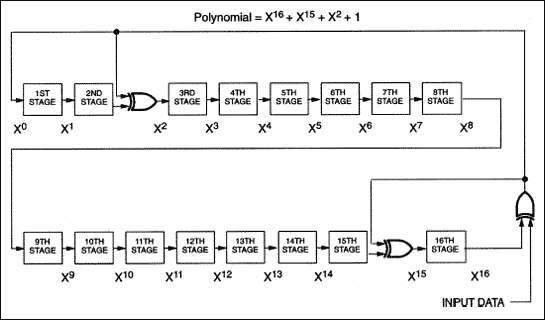
\includegraphics[scale=1]{\CURPATH/CRC16.png}
\caption{}
\end{figure}

( The source of image: \url{https://olimex.wordpress.com/2014/01/10/weekend-programming-challenge-week-39-crc-16/} )

Only 3 XOR gates are present aside of shift register.

The following page has animation: \url{https://en.wikipedia.org/wiki/Computation_of_cyclic_redundancy_checks}.

It can be implemented maybe even using vacuum tubes.

And the task is not to compute remainder according to rules of arithmetics, but rather to detect errors.

Compare this to a division circuit with at least one binary adder/subtractor, which will have carry-ripple problem.
On the other hand, addition over GF(2) has no carries, hence, this problem absent.

\myheading{Further reading}

These documents I've found interesting/helpful:

\begin{itemize}

\item \url{http://www.ross.net/crc/download/crc_v3.txt}
\item \url{https://www.kernel.org/doc/Documentation/crc32.txt}
\item \url{http://web.archive.org/web/20161220015646/http://www.hackersdelight.org/crc.pdf}

\end{itemize}

\levelup{}


\newchapter{Logarithms}

\leveldown{}

\myheading{Introduction}

\leveldown{}

\myheading{Children's approach}

When children argue about how big their favorite numbers are, they speaking about how many zeroes it has:
``$x$ has $n$ zeroes!''
``No, my $y$ is bigger, it has $m>n$ zeroes!''

This is exactly notion of common (base 10) logarithm.

Googol ($10^{100}$) has 100 zeroes, so $log_{10} (googol) = 100$.

Let's take some big number, like 12th Mersenne prime:

\begin{lstlisting}[caption=Wolfram Mathematica]
In[]:= 2^127 - 1
Out[]= 170141183460469231731687303715884105727
\end{lstlisting}

Wow, it's so big. How can we measure it in childish terms? How many digits it has? We can count using common (base 10) logarithm:

\begin{lstlisting}[caption=Wolfram Mathematica]
In[]:= Log[10, 2^127 - 1] // N
Out[]= 38.2308
\end{lstlisting}

So it has 39 digits.

Another question, how may decimal digits 1024-bit RSA key has?

\begin{lstlisting}[caption=Wolfram Mathematica]
In[]:= 2^1024
Out[]= 17976931348623159077293051907890247336179769789423065727343008\
1157732675805500963132708477322407536021120113879871393357658789768814\
4166224928474306394741243777678934248654852763022196012460941194530829\
5208500576883815068234246288147391311054082723716335051068458629823994\
7245938479716304835356329624224137216

In[]:= Log10[2^1024] // N
Out[]= 308.255
\end{lstlisting}

309 decimal digits.

\myheading{Scientists' and engineers' approach}

Interestingly enough, scientists' and engineers' approach is not very different from children's.
They are not interesting in noting each digit of some big number, they are usually interesting in three properties of some number:
1) sign; 2) first $n$ digits (significand or mantissa); 3) exponent (how many digits the number has).

The common way to represent a real number in handheld calculators and FPUs is:

\begin{equation}
(sign) significand \times 10^{exponent}
\end{equation}

For example:

\begin{equation}
-1.987126381 \times 10^{41}
\end{equation}

It was common for scientific handheld calculators to use the first ~10 digits of significand and ignore everything behind.
Storing the whole number down to the last digit is 1) very expensive; 2) hardly useful.

The number in IEEE 754 format (most popular way of representing real numbers in computers) has these three parts, however, 
it has different base (2 instead of 10).

\levelup{}


\myheading{Logarithmic scale}

\leveldown{}

\myheading{In human perception}

Logarithmic scale is very natural to human perceptions, including eyes.
When you ask average human to judge on current lighting, he/she may use words like ``dark'', ``very dark'', ``normal'', ``twilight'', ``bright'', 
``like on beach''.
In human language, there are couple of steps between ``dark'' and ``bright'', but luminous intensity may differ by several orders of magnitude.
Old cheap ``point-n-shoot'' photo cameras also has scale expressed in natural human languages.
But professional photo cameras also has logarithmic scales:

\begin{figure}[H]
\centering
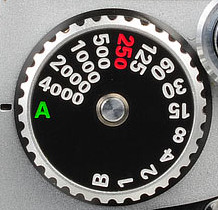
\includegraphics[scale=0.66]{log/nikon.jpg}
\caption{Shutter speed ($\frac{1}{x}$ of second) knob on photo camera}
\end{figure}

Another logarithmic scale familiar to anyone is decibel.
Even on cheap mp3 players and smartphones, where the volume is measured in conventional percents, this scale is logarithmic, 
and the difference between 50\% and 60\% may be much larger in sound pressure terms.

Yet another familiar to anyone logarithmic scale is Richter magnitude scale
\footnote{\url{https://en.wikipedia.org/wiki/Richter_magnitude_scale}}.
The Richter scale is practical, because when people talk about earthquakes, they are not interesting in exact scientific values
(in Joules or TNT equivalent), they are interesting in how bad damage is.

\myheading{In electronics engineering}

The loudspeakers are not perfect, so its output is non-linear in relation to input frequency.
In other word, loudspeaker has different loudness at different frequency.
It can be measured easily, and here is an example of plot of some speaker, I took it there:
\url{http://www.3dnews.ru/270838/page-3.html}.

\begin{figure}[H]
\centering
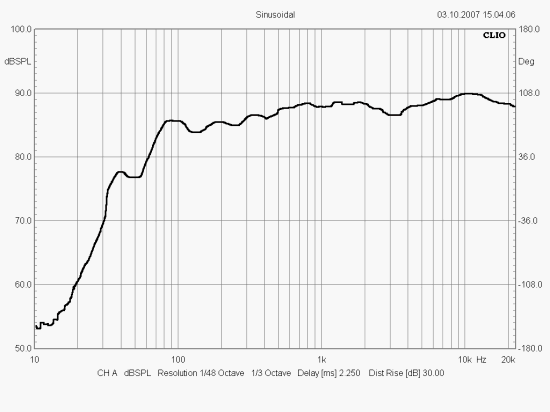
\includegraphics[scale=0.66]{log/65366.png}
\caption{Frequency response (also known as \textit{Bode plot}) of some loudspeaker}
\end{figure}

Both axis on this plot are logarithmic: y axis is loudness in decibel and x axis is frequency in Hertz.
Needless to say, the typical loudspeaker has bass/medium speaker + tweeter (high frequency speaker).
Some of more advanced loudspeaker has 3 speakers: bass, medium and tweeter.
Or even more.
And since the plot is logarithmic, each of these 2 or 3 speakers has their own part of plot, and these parts has comparable size.
If the x axis would be linear instead of logarithmic, the main part of it would be occupied by frequency response of tweeter alone, 
because it has widest frequency range. While bass speaker has narrowest frequency range, it would have very thin part of the plot.

y axis (vertical) of the plot is also logarithmic (its value is shown in decibels).
If this axis would be linear, the main part of it would be occupied by very loud levels of sound, while there would be thinnest line at the bottom
reserved for normal and quiet level of sounds.

Both of that would make plot unusable and impractical.
So both axis has logarithmic scale.
In strict mathematics terms, the plot shown is called \textit{log-log plot}, which means that both axis has logarithmic scale.

Summarizing, both electronics engineers and HiFi audio enthusiasts use these plots to compare quality of speakers.
These plots are often used in loudspeakers reviews
\footnote{Some of speakers of USSR era (like Latvian Radiotehnika S-30 and S-90) 
had such plots right on the surface of speaker box, presumably, for marketing purposes.}.

\myheading{In IT}

git, like any other VCS, can show a graph, how many changes each file got in each commit, for example:

\lstinputlisting{log/git_log.txt}

This scale is not logarithmical (I had a look into git internals), but this is exact place where logarithmical scale can be used.
When software developer got such report, he/she don't interesting in exact numbers of lines changed/added/removed.
He/she wants to see an outlook: which files got most changes/additions/removals, and which got less.

There is also a constraint: the space on the terminal is limited, so it's not possible to draw a minus or plus sign for each changed line of code.

Another example is Bitcoin client ``signal reception strength'', apparently, modeled after mobile phone signal indicator:

\begin{figure}[H]
\centering

\includegraphics[scale=1]{log/bitcoin_bars.png}
\caption{Bitcoin client}
\end{figure}

These bars indicating, how many connections client currently has.
Let's imagine, client can support up to 1000 connections, but user is never interesting in precise number, all he/she wants to know is how good its link
with Bitcoin network is.
I don't know how Bitcoin calculates this, but I think one bar could indicate that client has only 1 connection, two bars --- 2-5, three bars --- up to 10-20,
and four bars --- anything bigger.
This is also logarithmic scale.
On contrary, if you divide 1000 by 4 even parts, and one bar will fired if you've got 250 connections, two bars if you've got 500, etc, 
this would make the indicator useless, such indicators are no better than simple ``on/off'' lamp.

\myheading{Web 2.0}

Sites like GitHub, Reddit, Twitter sometimes shows how long some event was ago, instead of precise date (at least in 2015).
For example, Reddit may show date as ``3 years ago'', ``11 months ago'', ``3 weeks ago'', ``1 day ago'', ``10 hours ago'', etc, down to minutes and seconds.
You wouldn't see ``3 years and 11 hours ago''.
This is also logarithmic scale.
When some event happens 10 months ago, users are typically not interesting in precision down to days and hours.
When something happens 2 years ago, users usually not interesting in number of months and days in addition to these 2 years.

\levelup{}


\section{Multiplication and division using addition and subtraction}

It is possible to use addition instead of multiplication, using the following rule:

\begin{equation} \label{eq:1}
\log_{base} (ab) = \log_{base} (a) + \log_{base}(b)
\end{equation}

\dots while base can be any number.

It's like summing number of zeroes of two numbers. Let's say, you need to multiply 100 by 1000. Just sum number of their zeroes (2 and 3).
The result if the number with 5 zeroes. It's the same as $\log_{10} (100) + \log_{10} (1000) = \log_{10} (100000)$.

Division can be replaced with subtraction in the very same way.

\subsection{Logarithmic slide rule}

Here is very typical slide rule\footnote{I took screenshots at \url{http://museum.syssrc.com/static/sliderule.html}}.
It has many scales, but take a look on C and D scales, they are the same:

\begin{figure}[H]
\centering
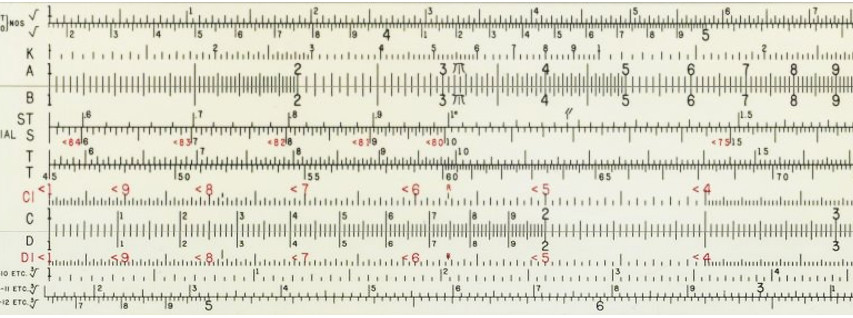
\includegraphics[scale=0.66]{log/sliderule1.jpg}
\caption{Initial state of slide rule}
\end{figure}

Now shift the core of rule so C scale at 1 will point to 1.2 at D scale:

\begin{figure}[H]
\centering
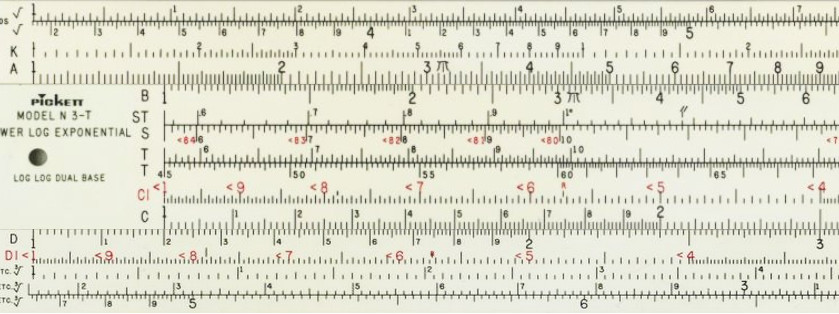
\includegraphics[scale=0.66]{log/sliderule2.jpg}
\caption{C scale shifted}
\end{figure}

% TODO дорисовать стрелки как в https://commons.wikimedia.org/wiki/File:Slide_rule_example2_with_labels.svg?uselang=ru

Find 2 at C scale and find corresponding value at D scale (which is 2.4).
Indeed, $1.2 \cdot 2 = 2.4$.
It works because by sliding scales we actually add distance between 1 and 1.2 (at any scale) to the distance between 1 and 2 (at any scale).
But since these scales logarithmic, addition of logarithmic values is the same as multiplication.

Values on scales can be interpreted as values of other order of magnitude.
We can say that 1 at C scale is actually point to 12 at D scale.
Find 1.8 at D scale (which is 18 now), it points somewhere between 21 and 22.
It's close: $12 \cdot 18 = 216$.

It works because of equation \ref{eq:1}.

Here is another example from Wikipedia:

\begin{figure}[H]
\centering
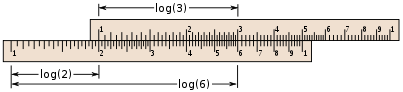
\includegraphics[scale=0.66]{log/403px-Slide_rule_example2_with_labels.svg.png}
\caption{Example from Wikipedia}
\end{figure}

\subsection{Logarithmic tables}

As we can see, the precision of logarithmic slide rule is up to 1 or 2 decimal digits after point.
Using precomputed logarithmic tables, it's possible to calculate product of two numbers with a precision up to $\approx 4$ digits.

First, find common (base of 10) logarithms of each number using logarithmic table:

\begin{figure}[H]
\centering
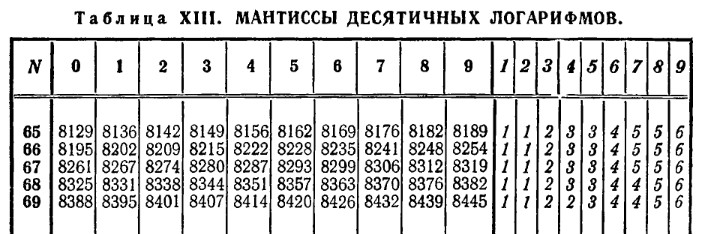
\includegraphics[scale=0.66]{log/bradis1.jpg}
\caption{Logarithmic tables}
\end{figure}

Then add these numbers. Find the number you got in table of powers of 10 ($10^{x}$, also called ``anti-log table''):

\begin{figure}[H]
\centering
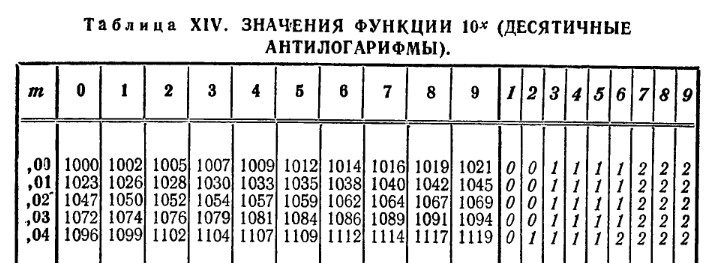
\includegraphics[scale=0.66]{log/bradis2.jpg}
\caption{Antilog tables}
\end{figure}

% TODO CRC book! спросить у него? http://www.mathtable.com/smtf/

Resulting number is a product.
The whole process may be faster than to multiply using long multiplication method using paper-n-pencil taught in schools.

Screenshots I took from the Bradis' book, once popular in USSR.
Another well-known book in western world with logarithmic and other tables is 
Daniel Zwillinger - CRC Standard Mathematical Tables and Formulae 
(up to 30th edition, the logarithmic tables are dropped after).

\subsection{Working with very small and very large numbers}

It's hard to believe, but the rule used on logarithmic slide rule for multiplication is still used sometimes in software code.
It's a problem to work with very small (denormalized) numbers
\footnote{Denormalized numbers in double-precision floating point format are numbers between $\approx 10^{324}$ and $\approx 10^{308}$} encoded in IEEE 754 standard. 

Here is my attempt to calculate $\frac{1.234 \times 10^{-300} \cdot 2.345678901234 \times 10^{-24}}{3.456789 \times 10^{-50}}$:

\begin{lstlisting}[caption=C code]
#include <stdio.h>
#include <math.h>

int main()
{
	double a=1.234e-300;
	double b=2.345678901234e-24;
	double c=3.456789e-50;
	printf ("%.30e\n", a*b/c);
};
\end{lstlisting}

The output is $1.429261797122261460966983388190 \times 10^{-274}$, which is incorrect.
When using debugger, we can see that the multiplication operation raises \textit{inexact exception} and \textit{underflow exception} in FPU.
The division operation also raises \textit{inexact exception}.

Let's check in Wolfram Mathematica:

\begin{lstlisting}[caption=Wolfram Mathematica]
In[]:= a = 1.234*10^(-300);

In[]:= b = 2.345678901234*10^(-24);

In[]:= c = 3.456789*10^(-50);

In[]:= a*b/c
Out[]= 8.37357*10^-275
\end{lstlisting}

The underflow exception raised in my C program because result of multiplication is in fact 
$2.894567764122756*10^{-324}$, which is even smaller than smallest denormalized number FPU can work with.

Let's rework our example to compute it all using natural logarithms 
(\texttt{exp(x)} is a C standard function, which computes $e^x$ and \texttt{log(x)} here is $\log_e(x)$ (or $ln(x)$)):

\begin{lstlisting}[caption=C code]
#include <stdio.h>
#include <math.h>

int main()
{
	double a=1.234e-300;
	double b=2.345678901234e-24;
	double c=3.456789e-50;
	printf ("%.30e\n", exp(log(a)+log(b)-log(c)));
};
\end{lstlisting}

Now the output is $8.373573753338710216281125792150 \times 10^{-275}$, same as Mathematica reported.

The same problem with very large numbers.

\begin{lstlisting}[caption=C code]
#include <stdio.h>
#include <math.h>

int main()
{
	double a=1.234e+300;
	double b=2.345678901234e+24;
	double c=3.456789e+50;
	printf ("%.30e\n", a*b/c);
};
\end{lstlisting}

When this program running, its result is ``inf'', meaning $\infty$, i.e., overflow occurred.
When using debugger, we can see than the multiplication operation raises \textit{inexact exception} plus \textit{overflow exception}.
The correct value in Wolfram Mathematica is...

\begin{lstlisting}[caption=Wolfram Mathematica]
In[]:= a = 1.234*10^300;

In[]:= b = 2.345678901234*10^24;

In[]:= c = 3.456789*10^50;

In[]:= a*b/c
Out[]= 8.37357*10^273
\end{lstlisting}

Let's rewrite our C example:

\begin{lstlisting}[caption=C code]
int main()
{
	double a=1.234e+300;
	double b=2.345678901234e+24;
	double c=3.456789e+50;
	printf ("%.30e\n", exp(log(a)+log(b)-log(c)));
};
\end{lstlisting}

Now the program reports $8.373573753337712538419923350878 \times 10^{273}$, which is correct value.

The way of representing all numbers as their logarithms called ``logarithmic number system''
\footnote{\url{https://en.wikipedia.org/wiki/Logarithmic_number_system}}.
It allows to work with numbers orders of magnitude lower than FPU can handle.

So why all computations are not performed using logarithms, if it's so good?
It's better only for very small or very large numbers.
Working with small and medium numbers, precision of its logarithmic versions will be much more important and harder to control.

Also, finding logarithm of a number with the following exponentiation are operations may be slower than multiplication itself.

\subsection{IEEE 754: adding and subtracting exponents}

IEEE 754 floating point number consists of sign, significand and exponent.
Internally, its simplified representation is:

\begin{equation}
(-1)^{sign} \cdot significand \times 2^{exponent}
\end{equation}

Given that, the FPU may process significands and exponents separately during multiplication, 
but when it processes exponents of two numbers, they are just summed up.
For example:

\begin{equation}
significand_{1} \times 2^{10} \cdot significand_{2} \times 2^{50} = significand_{3} \times 2^{60}
\end{equation}

\dots precise values of significands are omitted, but we can be sure, if the first number has exponent of $10$, the second has $50$,
the exponent of the resulting number will be $\approx 60$.

Conversely, during division, exponent of divisor is subtracted from the exponent of the dividend.

\begin{equation}
\frac{significand_{1} \times 2^{10}}{significand_{2} \times 2^{50}} = significand_{3} \times 2^{-40}
\end{equation}

I don't have access to Intel or AMD FPU internals, but I can peek into OpenWatcom FPU emulator libraries
\footnote{It was a time in 1980s and 1990s, when FPU was expensive and it could be bought separately 
in form of additional chip and added to x86 computer.
And if you had run a program which uses FPU on the computer where it's missing, FPU emulating library might be an option.
Much slower, but better than nothing.}.

Here is summing of exponents during multiplication:\\
\url{https://github.com/open-watcom/open-watcom-v2/blob/86dbaf24bf7f6a5c270f5a6a50925f468d8d292b/bld/fpuemu/386/asm/fldm386.asm\#L212}.\\
And here is subtracting of exponents during division:\\
\url{https://github.com/open-watcom/open-watcom-v2/blob/e649f6ed488eeebbc7ba9aeed8193d893288d398/bld/fpuemu/386/asm/fldd386.asm\#L237}.

Here is also multiplication function from FPU emulator in Linux kernel:
\url{https://github.com/torvalds/linux/blob/da957e111bb0c189a4a3bf8a00caaecb59ed94ca/arch/x86/math-emu/reg_u_mul.S\#L93}.

\subsection{Check, if the product will overflow}

Using logarithmic versions of two numbers, it is easy to check if the product of them will overflow in current environment (32-bit or 64-bit CPU registers).
Perhaps, programming languages with dynamic typing (like LISP, Python, Ruby, BASIC, etc) can check, 
if the current number must be switched to bignum (if the result is too big to fit in the CPU register) or not.



\myheading{Exponentiation}

Using equation \ref{eq:1} we may quickly notice that

\begin{equation}
b^n = \underbrace{b \times \cdots \times b}_n = base^{(\log_{base} (b))*n}
\end{equation}

That works with any logarithmic base.
In fact, this is the way how exponentiation is computed on computer.
x86 CPU and x87 FPU has no special instruction for it.

This is the way how pow() function works in Glibc: \url{https://github.com/lattera/glibc/blob/master/sysdeps/x86_64/fpu/e_powl.S\#L189}:\\

\begin{lstlisting}[caption={Glibc source code, fragment of the pow() function}]

...

7:	fyl2x			// log2(x) : y
8:	fmul	%st(1)		// y*log2(x) : y
	fst	%st(1)		// y*log2(x) : y*log2(x)
	frndint			// int(y*log2(x)) : y*log2(x)
	fsubr	%st, %st(1)	// int(y*log2(x)) : fract(y*log2(x))
	fxch			// fract(y*log2(x)) : int(y*log2(x))
	f2xm1			// 2^fract(y*log2(x))-1 : int(y*log2(x))
	faddl	MO(one)		// 2^fract(y*log2(x)) : int(y*log2(x))
	fscale			// 2^fract(y*log2(x))*2^int(y*log2(x)) : int(y*log2(x))
	fstp	%st(1)		// 2^fract(y*log2(x))*2^int(y*log2(x))

...

\end{lstlisting}

x87 FPU has the following instructions used Glibc's version of pow() function:
FYL2X (compute $y \cdot log_2 x$), F2XM1 (compute $2^x–1$).
Even more than that, FYL2X instruction doesn't compute binary logarithm alone, it also performs multiplication operation, 
to provide more easiness in exponentiation computation.

It works because calculating $2^x$ (exponentiation with base 2) is faster than exponentiation of arbitrary number.

Using hacker's tricks, it's also possible to take advantage of the IEEE 754 format and SSE instructions set:\\
\url{http://stackoverflow.com/a/6486630/4540328}.


\myheading{Square root}

Likewise, square root can be computed in the following way:

\begin{equation}
\sqrt[2]{x} = 2^{\frac{\log_2{x}}{2}}
\end{equation}

This leads to an interesting consequence: if you have a value stored in logarithmical form and you need to take
square root of it and leave it in logarithmical form, all you need is just to divide it by 2.

And since floating point numbers encoded in IEEE 754 has exponent encoded in logarithmical form,
you need just to shift it right by 1 bit to get square root:
\url{https://en.wikipedia.org/wiki/Methods_of_computing_square_roots#Approximations_that_depend_on_the_floating_point_representation}.

Likewise, cube root and nth root can be calculated using logarithm of corresponding base:

\begin{equation}
\sqrt[b]{x} = b^{\frac{\log_b{x}}{b}}
\end{equation}


\section{Base conversion}

FYL2X and F2XM1 instructions are the only logarithm-related x87 FPU has.
Nevertheless, it's possible to compute logarithm with any other base, using these.
The very important property of logarithms is:

\begin{equation}
\log_y (x) = \frac{\log_a (x)}{\log_a (y)}
\end{equation}

So, to compute common (base 10) logarithm using available x87 FPU instructions, we may use this equation:

\begin{equation}
\log_{10} (x) = \frac{\log_2 (x)}{\log_2 (10)}
\end{equation}

\dots while $\log_2(10)$ can be precomputed ahead of time.

Perhaps, this is the very reason, why x87 FPU has the following instructions:
FLDL2T (load $\log_2 (10)=3.32193...$ constant) and FLDL2E (load $\log_2 (e)=1.4427...$ constant).

Even more than that.
Another important property of logarithms is:

\begin{equation}
\log_y (x) = \frac{1}{\log_x (y)}
\end{equation}

Knowing that, and the fact that x87 FPU has FYL2X instruction (compute $y \cdot log_2 x$), logarithm base conversion can be done using multiplication:

\begin{equation}
\log_y (x) = \log_a (x) \cdot \log_y (a)
\end{equation}

So, computing common (base 10) logarithm on x87 FPU is:

\begin{equation}
\log_{10} (x) = \log_2 (x) \cdot \log_{10} (2)
\end{equation}

Apparently, that is why x87 FPU has another pair of instructions:

FLDLG2 (load $\log_{10} (2)=0.30103...$ constant) and FLDLN2 (load $\log_e (2)=0.693147...$ constant).

Now the task of computing common logarithm can be solved using just two FPU instructions: FYL2X and FLDLG2.

This piece of code I found inside of Windows NT4 ( \texttt{src/OS/nt4/private/fp32/tran/i386/87tran.asm} ), 
this function is capable of computing both common and natural logarithms: 

\begin{lstlisting}[caption=Assembly language code]
lab fFLOGm
        fldlg2                          ; main LOG10 entry point
        jmp     short fFYL2Xm

lab fFLNm                               ; main LN entry point
        fldln2

lab fFYL2Xm
        fxch
        or      cl, cl                  ; if arg is negative
        JSNZ    Yl2XArgNegative         ;    return a NAN
        fyl2x                           ; compute y*log2(x)
        ret
\end{lstlisting}



\myheading{Binary logarithm}

Sometimes denoted as lb(), binary logarithms are prominent in computer science, 
because numbers are usually stored and processed in computer in binary form.

\leveldown{}

\myheading{Denoting a number of bits for some value}

How many bits we need to allocate to store googol number ($10^{100}$)?

\begin{lstlisting}[caption=Wolfram Mathematica]
In[]:= Log2[10^100] // N
Out[]= 332.193
\end{lstlisting}

Binary logarithm of some number is the number of how many bits needs to be allocated.

If you have a variable which always has $2^x$ form, it's a good idea to store a binary logarithmic representation ($\log_2 (x)$) instead of it.
There are at least two reasons:
1) the programmer shows to everyone that the number has always $2^x$ form;
2) it's error-prone, it's not possible to accidentally store a number in some other form to this variable, so this is some kind of protection;
3) logarithmic representation is more compact.
There is, however, performance issue: the number must be converted back, but this is just one shifting operation (\texttt{1<<log\_n}).

Here is an example from NetBSD NTP client ( \texttt{netbsd-5.1.2/usr/src/dist/ntp/include/ntp.h} ):

\begin{lstlisting}[caption=C code]
/*
 * Poll interval parameters
 */
...
#define NTP_MINPOLL     4       /* log2 min poll interval (16 s) */
#define NTP_MINDPOLL    6       /* log2 default min poll (64 s) */
#define NTP_MAXDPOLL    10      /* log2 default max poll (~17 m) */
#define NTP_MAXPOLL     17      /* log2 max poll interval (~36 h) */
\end{lstlisting}

Couple examples from zlib (\texttt{deflate.h}):

\begin{lstlisting}[caption=C code]
    uInt  w_size;        /* LZ77 window size (32K by default) */
    uInt  w_bits;        /* log2(w_size)  (8..16) */
    uInt  w_mask;        /* w_size - 1 */
\end{lstlisting}

Another piece from zlib ( \texttt{contrib/blast/blast.c} ):

\begin{lstlisting}[caption=C code]
    int dict;           /* log2(dictionary size) - 6 */
\end{lstlisting}

If you need to generate bitmasks in range 1, 2, 4, 8...0x80000000, it is good idea to assign self-documenting name to iterator variable:

\begin{lstlisting}[caption=C code]
for (log2_n=1; log2_n<32; log2_n++)
    1<<log2_n;
\end{lstlisting}

Now about compactness, here is the fragment I found in OpenBSD, related to SGI IP22 architecture
\footnote{\url{http://www.linux-mips.org/wiki/IP22}} \\
( \texttt{OS/OpenBSD/sys/arch/sgi/sgi/ip22\_machdep.c} ):

\begin{lstlisting}[caption=C code]
                /*
                 * Secondary cache information is encoded as WWLLSSSS, where
                 * WW is the number of ways
                 *   (should be 01)
                 * LL is Log2(line size)
                 *   (should be 04 or 05 for IP20/IP22/IP24, 07 for IP26)
                 * SS is Log2(cache size in 4KB units)
                 *   (should be between 0007 and 0009)
                 */
\end{lstlisting}

Here is another example of using binary logarithm in Mozilla JavaScript engine (JIT compiler)
\footnote{\url{http://fossies.org/linux/seamonkey/mozilla/js/src/jit/mips/CodeGenerator-mips.cpp}}.
If some number is multiplied by $2^x$, the whole operation can be replaced by bit shift left.
The following code ( \texttt{js/src/jit/mips/CodeGenerator-mips.cpp} ), 
when translating multiplication operation into MIPS machine code, first, get assured if the number 
is really has $2^x$ form, then it takes binary logarithm of it and generates MIPS SLL instruction, which states for ``Shift Left Logical''.

\begin{lstlisting}[caption=Mozilla JavaScript JIT compiler (translating multiplication operation into MIPS bit shift instruction)]
bool
 CodeGeneratorMIPS::visitMulI(LMulI *ins)
 {
           default:
             uint32_t shift = FloorLog2(constant);
 
             if (!mul->canOverflow() && (constant > 0)) {
                 // If it cannot overflow, we can do lots of optimizations.
                 uint32_t rest = constant - (1 << shift);
 
                 // See if the constant has one bit set, meaning it can be
                 // encoded as a bitshift.
                 if ((1 << shift) == constant) {
                     masm.ma_sll(dest, src, Imm32(shift));
                     return true;
                 }

...

\end{lstlisting}

Thus, for example, $x=y \cdot 1024$ (which is the same as $x=y \cdot 2^{10}$) translates into $x=y<<10$.

\myheading{Calculating binary logarithm}

If all you need is integer result of binary logarithm ($abs(\log_2(x))$ or $\lfloor \log_2(x) \rfloor$), 
calculating is just counting all binary digits in the number minus 1.
In practice, this is the task of calculating leading zeroes.

Here is example from Mozilla libraries ( \texttt{mfbt/MathAlgorithms.h}
\footnote{\url{http://fossies.org/linux/seamonkey/mozilla/mfbt/MathAlgorithms.h}} ):

\begin{lstlisting}[caption=Mozilla libraries]
class FloorLog2<T, 4>
{
public:
   static uint_fast8_t compute(const T aValue)
   {
     return 31u - CountLeadingZeroes32(aValue | 1);
   }
 };

inline uint_fast8_t
 CountLeadingZeroes32(uint32_t aValue)
 {
   return __builtin_clz(aValue);
 }
\end{lstlisting}

Latest x86 CPUs has LZCNT (Leading Zeroes CouNT) instruction for that
\footnote{GNU \texttt{\_\_builtin\_clz()} function on x86 architecture can be thunk for LZCNT}, 
but there is also BSR (Bit Scan Reverse) instruction appeared in 80386, which can be used for the same purpose.
More information about this instruction on various architectures: \url{https://en.wikipedia.org/wiki/Find_first_set}.

There are also quite esoteric methods to count leading zeroes without this specialized instruction: \url{http://yurichev.com/blog/de_bruijn/}.

\myheading{O(log n) time complexity}

Time complexity\footnote{\url{https://en.wikipedia.org/wiki/Time_complexity}} is a measure of speed of a specific algorithm 
in relation to the size of input data.

O(1) -- time is always constant, to matter what size of input data. Simplest example is object getter -- it just returns some value.

O(n) -- time is linear, growing according to the size of input data. Simplest example is search for some value in the input array.
The larger array, the slowest search.

O(log n) -- time is logarithmic to the input data.
Let's see how this can be.

Let's recall child's number guessting game\footnote{\url{http://rosettacode.org/wiki/Guess_the_number}}.
One player think about some number, the other should guess it, offering various versions.
First player answers, is guessed number is larger or less.
Typical dialogue can be as the follows:

\begin{lstlisting}
-- I think of a number in 1..100 range.
-- Is it 50?
-- My number is larger.
-- 75?
-- It is lesser.
-- 63?
-- Larger.
-- 69?
-- Larger.
-- 72?
-- Lesser.
-- 71?
-- Correct.
\end{lstlisting}

Best possible strategy is to divide the range in halves.
The range is shorten at each step by half.
At the very end, the range has lenght of 1, and this is correct answer.
Maximal number of steps using the strategy described here are $\log_2(initial\_range)$.
In our example, initial range is 100, so the maximum number of steps is 6.64... or just 7.
If the initial range is 200, maximum number of steps are $\log_2(200)=7.6..$ or just 8. The number of steps increasing by 1 when the range is doubled.
Indeed, doubled range indicates that the guesser needs just one more step at the start, not more.
If the initial range is 1000, numbers of steps are $\log_2(1000)=9.96...$ or just 10.

This is exactly O(log n) time complexity.\\
\\
Now let's consider couple of practical real-world algorithms.
One interesting thing is that if the input array is sorted, and its size is known, and we need to find some value in it, the algorithm works exactly
in the same way as child's number guessing game!
The algorithm starts in the middle of array and compare the value there with the value sought-after.
Depending on the result (larger or lesser), the \textit{cursor} is moved left or right and operating range is decreasing by half.
This is called binary search\footnote{\url{https://en.wikipedia.org/wiki/Binary_search_algorithm}}, and there is the \texttt{bsearch()} function in 
standard C/C++ library\footnote{\url{http://en.cppreference.com/w/cpp/algorithm/bsearch}}.\\
\\
Here is how binary search is used in git: \url{https://www.kernel.org/pub/software/scm/git/docs/git-bisect.html}.\\
\\
Another prominent example in CS is binary trees. They are heavily used internally in almost any programming language, when you use set, map, dictionary, etc.

Here is a simple example with the following numbers (or keys) inserted into binary tree:
0, 1, 2, 3, 5, 6, 9, 10, 11, 12, 20, 99, 100, 101, 107, 1001, 1010.

\tikzset
{
  treenode/.style = {align=center, inner sep=0pt, text centered},
  key/.style = {treenode, circle, white, draw=black, fill=black, minimum size=2.0em, text width=2.0em},
  empty/.style = {treenode, rectangle, draw=black, minimum width=0.5em, minimum height=0.5em}
}

\begin{center}
\begin{tikzpicture}[->,>=stealth',
		level 1/.style={sibling distance=6cm},
		level 2/.style={sibling distance=2.7cm},
		level 3/.style={sibling distance=1.7cm},
		level 4/.style={sibling distance=0.7cm}] 
	\node [key] {10}
	child { node [key] {1} 
		child{ node [key] {0} 
		}
		child{ node [key] {5}
			child{ node [key] {3}
				child{ node[key] {2}}
				child{ node[empty] {}}
			}
			child{ node [key] {6}
				child{ node[empty] {}}
				child{ node[key] {9}}
			}
		}                            
	}
	child { node [key] {100}
		child { node [key] {20}
			child{ node [key] {12}
				child{ node[key] {11}}
				child{ node[empty] {}}
			}
			child{ node [key] {99}
			}
		}
		child{ node [key] {107}
			child{ node [key] {101}}
			child{ node [key] {1001}
				child{ node[empty] {}}
				child{ node[key] {1010}}
			}
		}
	}
	; 
\end{tikzpicture}
\end{center}


And here is how binary tree search works: put \textit{cursor} at the root. Now compare the value under it with the value sought-after.
If the value we are seeking for is lesser than the current, take a move into left node. If it's bigger, move to the right node.
Hence, each left descendant node has value lesser than in 
ascendant node.
Each right node has value which is bigger.
The tree must be rebalanced after each modification (I gave examples of it in my book about reverse engineering (\url{http://beginners.re/}, 51.4.4)).
Nevertheless, lookup function is very simple, and maximal number of steps is $\log_n(number\_of\_nodes)$.
We've got 17 elements in the tree at the picture, $\log_2(17)=4.08...$, indeed, there are 5 tiers in the tree.

\levelup{}


\section{Common (base 10) logarithms}

Also known as ``decimal logarithms''.
Denoted as \texttt{lg} on handheld calculators.

10 is a number inherently linked with human's culture, since almost all humans has 10 digits.
Decimal system is a result of it.
Nevertheless, 10 has no special meaning in mathematics and science in general.
So are common logarithms.

One notable use is a decibel logarithmic scale, which is based of common logarithm.

Common logarithms are sometimes used to calculate space for decimal number in the string or on the screen.
How many characters you should allocate for 64-bit number? 20, because $log_{10}(2^{64}) = 19.2...$.

Functions like \texttt{itoa()}\footnote{\url{http://www.cplusplus.com/reference/cstdlib/itoa/}}
(which converts input number to a string) can calculate output buffer size precisely, 
calculating common logarithm of the input number.


\myheading{Natural logarithm}

Natural logarith (denoted as \texttt{ln} on handheld calculators, and sometimes denoted just as \texttt{log})
is logarithm of base $e=2.718281828...$.
Where this constant came from?

\leveldown{}

\myheading{Savings account in your bank}

Let's say you make a deposit into bank, say, 100 dollars (or any other currency).
They offer 2.5\% per year (annual percentage yield).
This mean, you'll can get doubled amount of money (200 dollars) after 40 years.
So far so good.
But some banks offers compound interest.
Also called ``complex percent'' in Russian language, where ``complex'' in this phrase is closer to the word ``folded''.
This mean, after each year, they pretend you withdraw your money with interest, then redeposit them instantly.
Banks also say that the interest is recapitalized once a year.
Let's calculate final amount of money after 40 years:

\lstinputlisting[caption=Python code]{log/APY1.py}

\begin{lstlisting}
year= 0 amount at the end 102.5
year= 1 amount at the end 105.0625
year= 2 amount at the end 107.6890625
year= 3 amount at the end 110.381289063
...
year= 36 amount at the end 249.334869861
year= 37 amount at the end 255.568241608
year= 38 amount at the end 261.957447648
year= 39 amount at the end 268.506383839
\end{lstlisting}

The thing is that the final amount (268.50...) is aimed toward $e$ constant.

Now there is another bank, which offers to recapitalize your deposit each month.
We'll rewrite our script slightly:

\lstinputlisting[caption=Python code]{log/APY2.py}

\begin{lstlisting}
year= 0 month= 0 amount 100.208333333
year= 0 month= 1 amount 100.417100694
year= 0 month= 2 amount 100.626302988
year= 0 month= 3 amount 100.835941119
...
year= 39 month= 8 amount 269.855455383
year= 39 month= 9 amount 270.417654248
year= 39 month= 10 amount 270.981024361
year= 39 month= 11 amount 271.545568162
\end{lstlisting}

The final result is even closer to $e$ constant.

Let's imagine there is a bank which allows to recapitalize each day:

\lstinputlisting[caption=Python code]{log/APY3.py}

\begin{lstlisting}
year= 0 month= 0 day= 0 amount 100.006944444
year= 0 month= 0 day= 1 amount 100.013889371
year= 0 month= 0 day= 2 amount 100.02083478
year= 0 month= 0 day= 3 amount 100.027780671
...
year= 39 month= 11 day= 26 amount 271.762123927
year= 39 month= 11 day= 27 amount 271.780996297
year= 39 month= 11 day= 28 amount 271.799869977
year= 39 month= 11 day= 29 amount 271.818744968
\end{lstlisting}

The final amount of money is more closer to $e$ constant.

If to imagine some really crazy bank client who redeposit his deposit infinite number of times per each day, the final value after 40 years
would be $100 \cdot e$.
It's not possible in the real world, so the final amount is approaches this value, but is never equal to it.
Mathematically speaking, its limit is $100 \cdot e$.

\myheading{Exponential decay}

\leveldown{}

\myheading{Capacitor discharge}

% TODO redraw! ибо спизжено. https://en.wikipedia.org/wiki/Talk%3ARC_circuit#RC_Circuits
\begin{figure}[H]
\centering
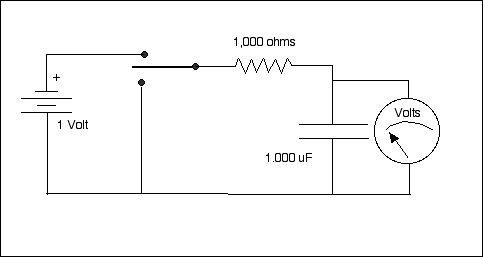
\includegraphics[scale=0.66]{log/Schematic_of_Battery_and_Capacitor.jpg}
\end{figure}

From electronics engineering course we may know that the capacitor discharging by half after $RC\ln(2)$ seconds,
where C is capacity of capacitor in farads and R resistance of resistor in ohms.
Given $1k\Omega$ resistor and $1000 \mu F$ capacitor, what its voltage after 1 seconds will be? after 2 seconds?
It's discharge can be calculated using this equation:

\LARGE\[
V=V_0 \cdot e^{\frac{-t}{RC}}
\]
\normalsize

\dots where $V_0$ is initial charge in volts, $t$ is time in seconds and $e$ is base of natural logarithm.

Let's see it in Wolfram Mathematica:

\begin{lstlisting}[caption=Wolfram Mathematica]
r = 1000; (* resistance in ohms *)

c = 0.001; (* capacity in farads *)

v = 1; (* initial voltage *)

Plot[v*E^((-t)/(r*c)), {t, 0, 5}, 
 GridLines -> {{Log[2], Log[2]*2, Log[2]*3}, {0.5, 0.25, 0.125}},
 Epilog -> {Text["ln(2)", {Log[2], 0.05}], 
   Text["ln(2)*2", {Log[2]*2, 0.05}], 
   Text["ln(2)*3", {Log[2]*3, 0.05}],
   Text["1/2", {0.1, 0.5}], Text["1/4", {0.1, 0.25}], 
   Text["1/8", {0.1, 0.128}]}, AxesLabel -> {seconds, voltage}]
\end{lstlisting}

\begin{figure}[H]
\centering
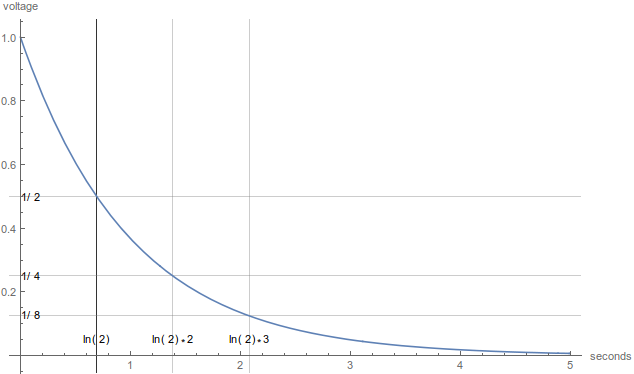
\includegraphics[scale=0.66]{log/capacitor_discharge.png}
\caption{Capacitor voltage during discharge}
\end{figure}

As we can see, $\frac{1}{2}$ of initial charge is left after $ln(2)$ seconds (~0.69...), 
and $\frac{1}{4}$ of charge is left after $ln(4)$ seconds (~1.38...).

Indeed, if we interesting in precise time in seconds, when charge will be $\frac{1}{x}$, just calculate $ln(x)$.

Now here is the same plot, but I added two more labels, $\frac{1}{3}$ and $\frac{1}{7}$:

\begin{lstlisting}[caption=Wolfram Mathematica]
Plot[v*E^((-t)/(r*c)), {t, 0, 5}, 
 GridLines -> {{Log[3], Log[7]}, {1/3, 1/7}},
 Epilog -> {Text["ln(3)", {Log[3], 0.05}], 
   Text["ln(7)", {Log[7], 0.05}],
   Text["1/3", {0.1, 1/3}], Text["1/7", {0.1, 1/7}]}, 
 AxesLabel -> {seconds, voltage}]
\end{lstlisting}

\begin{figure}[H]
\centering
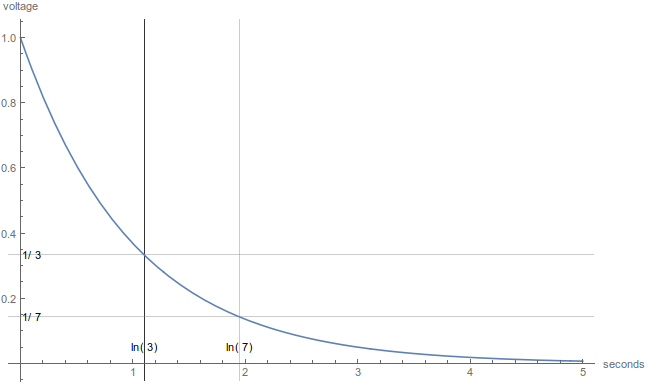
\includegraphics[scale=0.66]{log/capacitor_discharge2.png}
\caption{Capacitor voltage during discharge}
\end{figure}

\dots and we see that these points corresponds to $ln(3)$ and $ln(7)$.
That means, $\frac{1}{3}$ of charge is left after $ln(3) \approx 1.098...$ seconds and $\frac{1}{7}$ of charge after $ln(7) \approx 1.945...$ seconds.

\myheading{Radioactive decay}

Radioactive decay is also exponential decay.
Let's take Polonium 210 as an example\footnote{\url{https://en.wikipedia.org/wiki/Polonium}}.
It's half-life (calculated) is $\approx 138.376$ days.
That means that if you've got 1kg of Polonium 210, after $\approx 138$ days, half of it (0.5 kg) left as \textsuperscript{210}Po and 
another half is transformed into \textsuperscript{206}Pb (isotope of lead\footnote{\url{https://en.wikipedia.org/wiki/Isotopes_of_lead\#Lead-206}}).
After another $\approx 138$ days, you'll get $\frac{3}{4}$ of isotope of lead and $\frac{1}{4}$ will left as \textsuperscript{210}Po.
After another $\approx 138$ days, amount of Polonium will be halved yet another time, etc.

The equation of radioactive decay is:

\[
N=N_{0}e^{-\lambda t}
\]

\dots where $N$ is number of atoms at some point of time, $N_{0}$ is initial number of atoms, $t$ is time, $\lambda$ is decay constant.
Decay of Polonium is exponential, but decay constant is the constant, defining how fast (or slow) it will fall.

Here we go in Mathematica, let's get a plot for 1000 days:

\begin{lstlisting}[caption=Wolfram Mathematica]
l = 0.005009157516910051; (* decay constant of Polonium 210 *)

hl = Log[2]/l
138.376

Plot[E^(-l*t), {t, 0, 1000}, 
 GridLines -> {{hl, hl*2, hl*3}, {0.5, 0.25, 0.125}}, 
 Epilog -> {Text["hl", {hl, 0.05}], Text["hl*2", {hl*2, 0.05}], 
   Text["hl*3", {hl*3, 0.05}], Text["1/2", {30, 0.5}], 
   Text["1/4", {30, 0.25}], Text["1/8", {30, 0.128}]}, 
 AxesLabel -> {days, atoms}]
\end{lstlisting}

\begin{figure}[H]
\centering
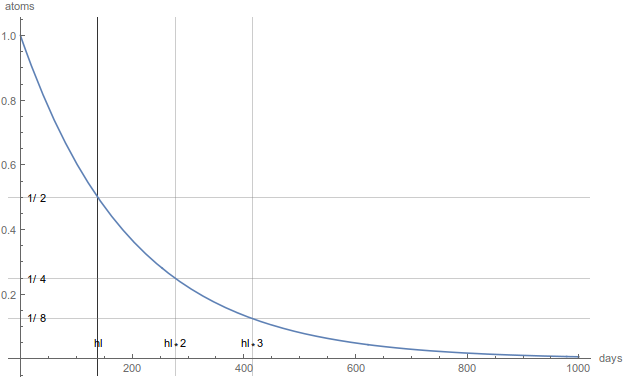
\includegraphics[scale=0.66]{log/210po.png}
\caption{Exponential decay of Polonium 210}
\end{figure}

\myheading{Beer froth}

There is even the paper (got Ig Nobel prize in 2002), author's of which demonstrates that beer froth is also decays exponentially:
\url{http://iopscience.iop.org/0143-0807/23/1/304/},
\url{https://classes.soe.ucsc.edu/math011a/Winter07/lecturenotes/beerdecay.pdf}.

\begin{figure}[H]
\centering
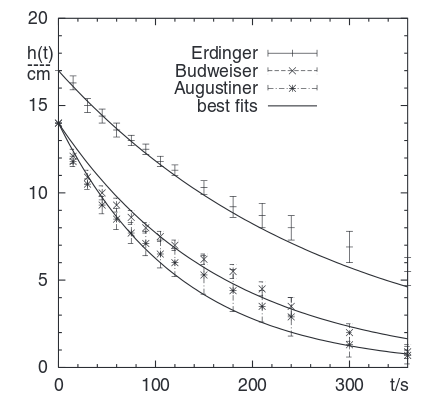
\includegraphics[scale=0.66]{log/beer.png}
\caption{Results from the paper}
\end{figure}

The paper can be taken as a joke, nevertheless, it's a good demonstration of exponential decay.

\myheading{Conclusion}

Capacitor discharge and radioactive decay obeys the same law of halving some amount after equal gaps of time:

\[
amount=amount_{0} \cdot e^{- decay\_constant \cdot time}
\]

Decay constant in case of capacitor discharge defined by product of resistance and capacity.
The bigger one of them, the slower decay.

Natural logarithm is used to calculate gap of time (half-life or half-time) judging by decay constant.

\levelup{}

\levelup{}


% TODO \section{Cheat sheet}

\levelup{}


\newchapter{Symbolic computation}

\leveldown{}

Some numbers can only be represented in binary system approximately, like $\frac{1}{3}$ and $\pi$.
If we calculate $\frac{1}{3} \cdot 3$ step-by-step, we may have loss of significance.
We also know that $sin(\frac{\pi}{2}) = 1$, but calculating this expression in usual way,
we can also have some noise in result.
Arbitrary-precision arithmetic\footnote{\url{https://en.wikipedia.org/wiki/Arbitrary-precision_arithmetic}} is not a solution,
because these numbers cannot be stored in memory as a binary number of finite length.

How we could tackle this problem?
Humans reduce such expressions using paper and pencil without any calculations.
We can mimic human behaviour programmatically if we will store expression as tree and symbols like $\pi$ will be converted into number at the very last step(s).

This is what Wolfram Mathematica\footnote{Another well-known symbolic computation system are 
\href{https://en.wikipedia.org/wiki/Maxima_\%28software\%29}{Maxima} and 
\href{https://en.wikipedia.org/wiki/SymPy}{SymPy}} does.
Let's start it and try this:

\begin{lstlisting}
In[]:= x + 2*8
Out[]= 16 + x
\end{lstlisting}

Since Mathematica has no clue what $x$ is, it's left \textit{as is}, but $2 \cdot 8$ can be reduced easily, both by Mathematica and by humans,
so that is what has done.
In some point of time in future, Mathematica's user may assign some number to $x$ and then, Mathematica will reduce the expression even further.

Mathematica does this because it parses the expression and finds some known patterns.
This is also called \textit{term rewriting}\footnote{\url{https://en.wikipedia.org/wiki/Rewriting}}.
In plain English language it may sounds like this:
``if there is a $+$ operator between two known numbers, replace this subexpression by a computed number which is sum of these two numbers, if possible''.
Just like humans do.

Mathematica also has rules like ``replace $sin(\pi)$ by 0'' and ``replace $sin(\frac{\pi}{2})$ by 1'', but as you can see, $\pi$ must be preserved
as some kind of symbol instead of a number.

% TODO example
So Mathematica left $x$ as unknown value.
This is, in fact, common mistake by Mathematica's users: a small typo in an input expression may lead to a huge irreducible expression with the typo left.

Another example: Mathematica left this deliberately while computing binary logarithm:

\begin{lstlisting}
In[]:= Log[2, 36]
Out[]= Log[36]/Log[2]
\end{lstlisting}

Because it has a hope that at some point in future, this expression will become a subexpression in another expression and 
it will be reduced nicely at the very end.
But if we really need a numerical answer, we can force Mathematica to calculate it:

\begin{lstlisting}
In[]:= Log[2, 36] // N
Out[]= 5.16993
\end{lstlisting}

Sometimes unresolved values are desirable:

\begin{lstlisting}
In[]:= Union[{a, b, a, c}, {d, a, e, b}, {c, a}]
Out[]= {a, b, c, d, e}
\end{lstlisting}

Characters in the expression are just unresolved symbols\footnote{\textit{Symbol} like in LISP} with no connections to numbers or other expressions, 
so Mathematica left them \textit{as is}.

Another real world example is symbolic integration\footnote{\url{https://en.wikipedia.org/wiki/Symbolic_integration}}, 
i.e., finding formula for integral by rewriting initial expression using some predefined rules.
Mathematica also does it:

\begin{lstlisting}
In[]:= Integrate[1/(x^5), x]
Out[]= -(1/(4 x^4))
\end{lstlisting}

Benefits of symbolic computation are obvious: it is not prone to loss of significance\footnote{\url{https://en.wikipedia.org/wiki/Loss_of_significance}} and 
round-off errors\footnote{\url{https://en.wikipedia.org/wiki/Round-off_error}}, but drawbacks are also obvious: you need to store expression in (possible huge) tree
and process it many times.
Term rewriting is also slow.
All these things are extremely clumsy in comparison to a fast \ac{FPU}.

``Symbolic computation'' is opposed to ``numerical computation'', the last one is just processing numbers step-by-step, using calculator, \ac{CPU} or \ac{FPU}.\\
\\
Some task can be solved better by the first method, some others -- by the second one.

\myheading{Rational data type}

Some LISP implementations can store a number as a ratio/fraction
\footnote{\url{https://en.wikipedia.org/wiki/Rational_data_type}}, i.e., placing two numbers in a cell (which, in this case, is called \textit{atom} in LISP lingo).
For example, you divide 1 by 3, and the interpreter, by understanding that $\frac{1}{3}$ is 
an irreducible fraction\footnote{\url{https://en.wikipedia.org/wiki/Irreducible_fraction}}, creates a cell with 1 and 3 numbers.
Some time after, you may multiply this cell by 6, and the multiplication function inside LISP interpreter may return much better result (2 without \textit{noise}).

Printing function in interpreter can also print something like \TT{1 / 3} instead of floating point number.

This is sometimes called ``fractional arithmetic'' [see \ac{TAOCP}, 3rd ed., (1997), 4.5.1, page 330].

This is not symbolic computation in any way, but this is slightly better than storing ratios/fractions as just floating point numbers.

Drawbacks are clearly visible: you need more memory to store ratio instead of a number;
and all arithmetic functions are more complex and slower, because they must handle both numbers and ratios.

Perhaps, because of drawbacks, some programming languages offers separate (\textit{rational}) data type, as language feature, or supported by a library
\footnote{More detailed list: \url{https://en.wikipedia.org/wiki/Rational_data_type}}:
Haskell, OCaml, Perl, Ruby, Python (\textit{fractions}), Smalltalk, Java, Clojure,
C/C++\footnote{By GNU Multiple Precision Arithmetic Library}.

\levelup{}


\newchapter{Graph theory}

\leveldown{}

Graph is a group of nodes, some of them may be connected with each other, some are not.
One of the popular examples is the map of country: there are cities and roads.
"Cities" are called "nodes" or "vertices" in mathematics lingo, while "roads" are called "edges".
Another popular example of graph is computer network, including Internet.
Computer network is graph indeed, but it's closer to "sparse graph", because for the most part, computer networks are trees.

\myheading{Clique in graph theory}

\leveldown{}

\renewcommand{\CURPATH}{graph/clique}

"Clique" in everyday speech (especially in political news) denotes a tight-knit group of people inside of some community.
In graph theory, "clique" is a subgraph (part of graph) each vertices ("nodes" or "members") of which are connected with each other.

\myheading{Social graph: simple example}

"Social graph" is a graph representing social links.
Here is example I made in Wolfram Mathematica:

\begin{lstlisting}
community = 
 Graph[{John <-> Mark, John <-> Alice, Mark <-> Alice, Tim <-> Alice, 
   Matthew <-> John, Matthew <-> Mark, Tim <-> John, Drake <-> Tim, 
   Bob <-> Drake, Bill <-> Mark, Bob <-> Alice, Tim <-> Mark}, 
  VertexLabels -> "Name"]
\end{lstlisting}

\begin{figure}[H]
\centering
\frame{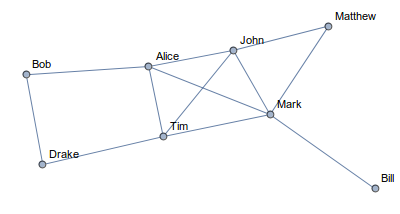
\includegraphics[scale=0.7]{\CURPATH/graph1.png}}
\end{figure}

Let's try to find largest clique:

\begin{lstlisting}
In[]:= clique = FindClique[community]
Out[]= {{John, Mark, Alice, Tim}}
\end{lstlisting}

Indeed, each of these four persons is connected to each among other 3.
Wolfram Mathematica can highlight subgraph in graph:

\begin{lstlisting}
HighlightGraph[community, clique]
\end{lstlisting}

\begin{figure}[H]
\centering
\frame{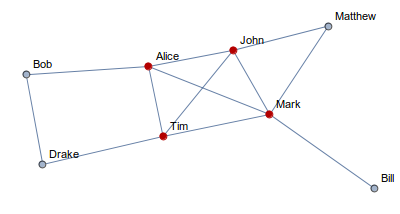
\includegraphics[scale=0.7]{\CURPATH/graph2.png}}
\end{figure}

\myheading{Social graph: IRC network}

Internet Relay Chat (IRC) is popular among open-source developers.
One of the most popular IRC networks is Freenode.
And one of the most crowded IRC channel there is \#ubuntu, devoted to Ubuntu Linux.
I used data from it, because all logs are available (starting at 2004), for example:
\url{http://irclogs.ubuntu.com/2015/01/01/%23ubuntu.txt}.

When someone asks, and someone another going to answer the question, IRC users are address each other in this way:

\begin{lstlisting}
[00:11] <synire> How would one find the path of an application installed using terminal?
[00:11] <zykotick9> synire: "whereis foo"
[00:11] <synire> zykotick9: thanks!
\end{lstlisting}

It's not a rule, but well-established practice, so we can recover the information, which users talks to which users most often.
Let's say, we would build a link between two IRC users if 
1) they talk to each other at least 10-11 days (not necessary consequent);
2) do this at least 6 months (not necessary consequent).

The largest cliques of \#ubuntu IRC channel in 10-11 years period are these:

\begin{lstlisting}
* clique size 11
['ubottu', 'ActionParsnip', 'ikonia', 'Ben64', 'zykotick9', 'theadmin', 'dr_willis', 'MonkeyDust', 'usr13', 'bekks', 'iceroot']
* clique size 10
['ubottu', 'ActionParsnip', 'ikonia', 'jrib', 'bazhang', 'Pici', 'iceroot', 'theadmin', 'IdleOne', 'erUSUL']
* clique size 10
['ubottu', 'ActionParsnip', 'ikonia', 'jrib', 'bazhang', 'Pici', 'iceroot', 'theadmin', 'zykotick9', 'usr13']
* clique size 10
['ubottu', 'ActionParsnip', 'ikonia', 'jrib', 'bazhang', 'Pici', 'iceroot', 'sebsebseb', 'IdleOne', 'erUSUL']
* clique size 10
['ubottu', 'ActionParsnip', 'ikonia', 'jrib', 'Dr_Willis', 'Pici', 'edbian', 'IdleOne', 'Jordan_U', 'theadmin']
* clique size 10
['ubottu', 'ActionParsnip', 'ikonia', 'jrib', 'Dr_Willis', 'Pici', 'edbian', 'IdleOne', 'Jordan_U', 'sebsebseb']
* clique size 10
['ubottu', 'ActionParsnip', 'ikonia', 'jrib', 'Dr_Willis', 'Pici', 'erUSUL', 'iceroot', 'IdleOne', 'theadmin']
* clique size 10
['ubottu', 'ActionParsnip', 'ikonia', 'jrib', 'Dr_Willis', 'Pici', 'erUSUL', 'iceroot', 'IdleOne', 'sebsebseb']
* clique size 10
['ubottu', 'ActionParsnip', 'ikonia', 'jrib', 'Dr_Willis', 'Pici', 'erUSUL', 'iceroot', 'ubuntu', 'sebsebseb']
* clique size 10
['ubottu', 'ActionParsnip', 'ikonia', 'Ben64', 'histo', 'bekks', 'MonkeyDust', 'dr_willis', 'iceroot', 'usr13']
...
\end{lstlisting}

% FIXME
Perhaps, these users are frequenters of the channel. List of all cliques are here:
\url{\GitHubBlobMasterURL/\CURPATH/files/IRC/results.txt}.
The output is not terse, because all listed cliques are cliques indeed, and single user or users group can be member of several cliques, that's correct.
Cliques can be overlapped and be members of bigger cliques.
It's possible to produce more human-like results using 
\href{https://en.wikipedia.org/wiki/Community_structure#Algorithms_for_finding_communities}{more complex algorithms for finding communities}.

The source code of my scripts here: \url{\GitHubTreeMasterURL/\CURPATH/files/IRC}.
I used the excellent \href{https://networkx.github.io/}{networkx graph library}.

\myheading{Attempt to find communities in IRC social graph}

Wolfram Mathematica can try to find communities within social graph.
Here I will import information about all IRC interactions from the start of 2013 till the summer of 2015.
User nicknames are coded by numbers for simplicity.

\begin{lstlisting}
In[]:= g2 = 
 Graph[{91708 -> 93574, 93414 -> 91525, 93414 -> 89579, 
   90407 -> 93896, 93414 -> 93598, 93809 -> 5909, 93698 -> 93801, 
   93163 -> 83317, 84930 -> 93896, 93414 -> 92947, 93414 -> 91708, 
   93792 -> 92887, 84930 -> 91708, 91708 -> 84930, 88400 -> 93698, 
   ...
   93809 -> 93475, 93698 -> 92887, 93801 -> 93670, 92887 -> 93598}]
\end{lstlisting}

The resulting graph is:

\begin{figure}[H]
\centering
\frame{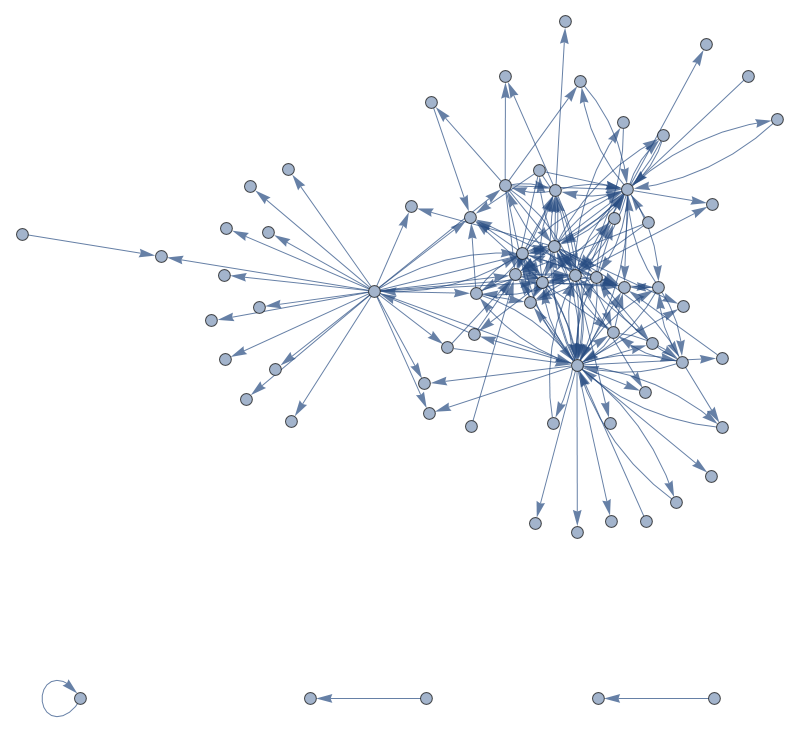
\includegraphics[scale=0.5]{\CURPATH/IRC_g2.png}}
\end{figure}

There some artifacts (at the bottom) which can be ignored so far, I think.
There is prominent centers: one huge and two others are smaller.
I'm not sure, but I can suggest these parts of graph are just users who has different sleep paterns, or, more likely, from different time zones,
so each important time zone (like Americas, Europe, Asia/Oceania) may have their own social communities.
But again, I'm not sure, this should be investigated first.

Let's try to find communities and hightlight them within the graph:

\begin{lstlisting}
c2 = FindGraphCommunities[g2];
HighlightGraph[g2, Map[Subgraph[g2, #] &, c2]]
\end{lstlisting}

\begin{figure}[H]
\centering
\frame{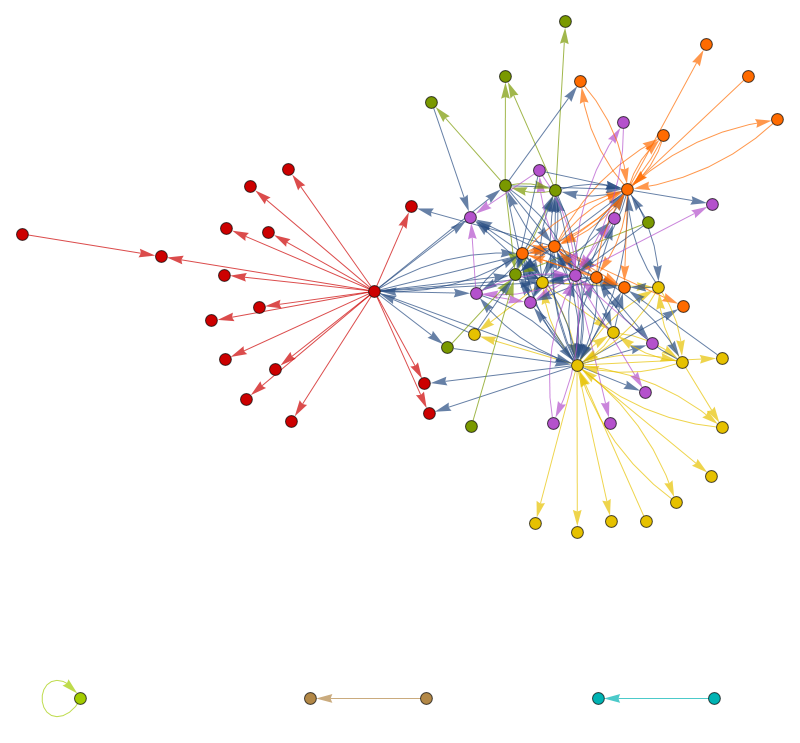
\includegraphics[scale=0.5]{\CURPATH/IRC_c2.png}}
\end{figure}

Hard to say if Mathematica right, but this is what it did.

Now let's take the whole graph of all IRC interactions starting at year 2004 till the summer of 2015.
The graph is much bigger:

\begin{figure}[H]
\centering
\frame{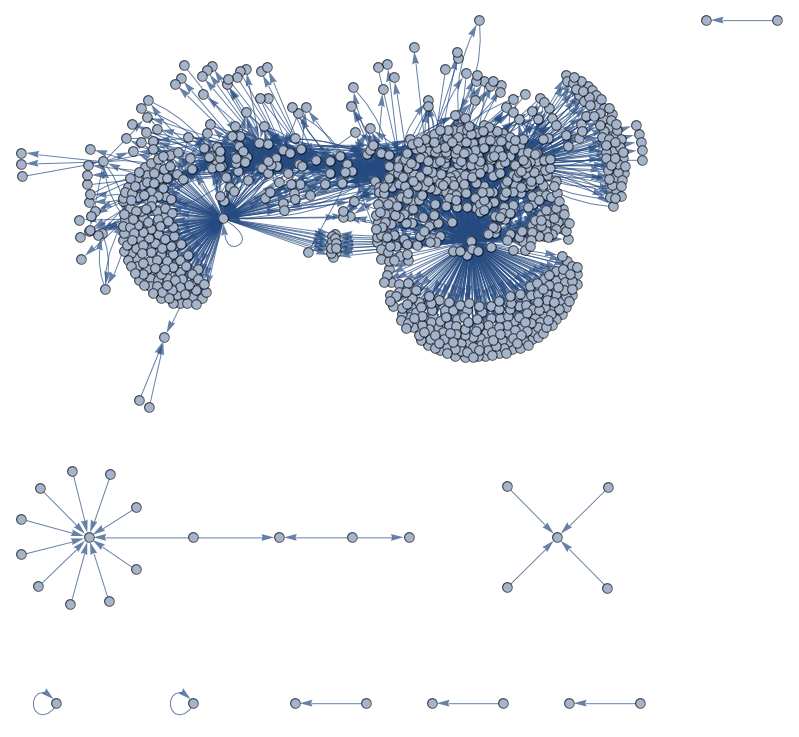
\includegraphics[scale=0.5]{\CURPATH/IRC_g1.png}}
\end{figure}

There are more artifacts.

Let's apply Mathematica's method to find communities:

\begin{figure}[H]
\centering
\frame{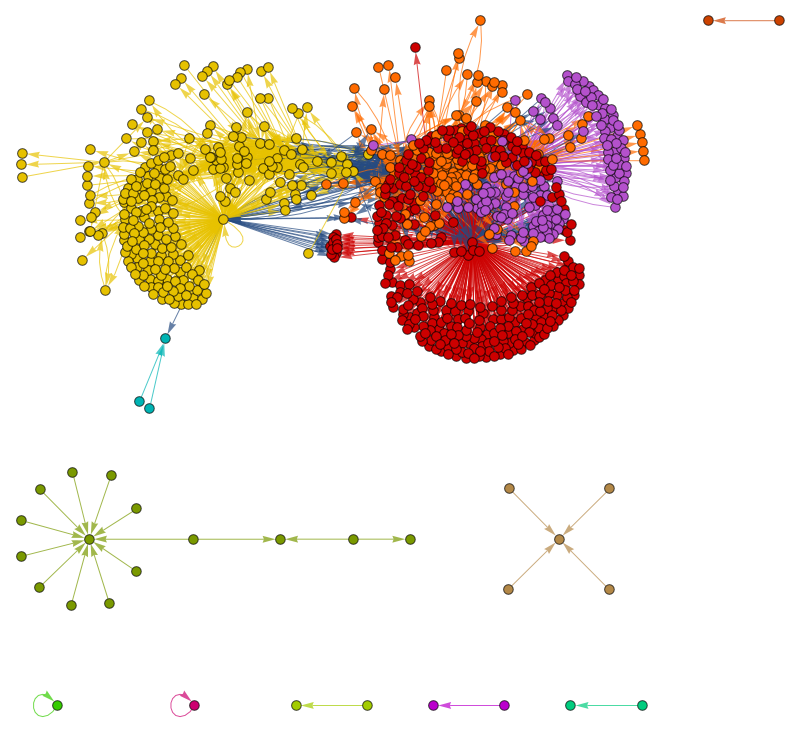
\includegraphics[scale=0.5]{\CURPATH/IRC_c1.png}}
\end{figure}

Is it right? Maybe. Needless to say, since timespan is so long (at least 10 years), we can belive that some communities which may exists in 2004-2006 may be
extinct in 2014-2015 (people got older, lost their interest in Ubuntu Linux, etc), but they all are visible on this graph.

Summary: perhaps, on our next experiment we should filter out IRC data by years and time zones.

\myheading{Social graph: social networks}

Perhaps, social networking websites like Facebook and Twitter in the "people you may know" tab shows you users of most populous (by your current friends) cliques.
It may be much more complex in reality, but nevertheless, this is simplest possible way to offer you new social contacts.

\myheading{Links graph: Wikipedia}

Wikipedia has a lot of internal links, ~463,000,000 in English Wikipedia as of summer 2015, if not to count user/talk/media pages, etc.
It's possible to build a graph where Wikipedia article is a vertice (or node) and a link from one article to another is edge.
By link between articles we would call the case when the first article has the link to the second article, but also the second has the link to the first one.

Here are some examples of cliques I found this way. Number in parenthesis is clique size.

\begin{itemize}

\item
Chess-related articles (9): Reuben Fine, Mikhail Botvinnik, Samuel Reshevsky, Max Euwe, FIDE, Alexander Alekhine, World Chess Championship, José Raúl Capablanca, AVRO 1938 chess tournament.

\item
Utah-related articles (9): Red Line (TRAX), Utah Transit Authority, Blue Line (TRAX), TRAX (light rail), Salt Lake City, Green Line (TRAX), FrontRunner, University of Utah, Utah.

\item
Articles related to Doctor Who (9): Doctor Who (film), Doctor Who, The Doctor (Doctor Who), Eighth Doctor, The Master (Doctor Who), Gallifrey, TARDIS, Doctor Who Magazine, Seventh Doctor.

\item
Space (9): New Horizons, Pioneer 11, Voyager 1, Europa (moon), Callisto (moon), Ganymede (moon), Jupiter, Io (moon), Pioneer 10.

\item
Hip hop music (9): G-funk, Dr. Dre, Death Row Records, Snoop Dogg, The Chronic, Gangsta rap, West Coast hip hop, N.W.A, Hip hop music.

\item
Metal music (9): Master of Puppets, Thrash metal, Cliff Burton, James Hetfield, Kirk Hammett, Metallica, Kill 'Em All, Ride the Lightning, Dave Mustaine.

\item
The Beatles (8): Break-up of the Beatles, The Beatles, George Harrison, Let It Be, John Lennon, Paul McCartney, Ringo Starr, Abbey Road.

\end{itemize}

Each Wikipedia article within any of these cliques has links to each article in clique.

Full lists of first 1000 largest cliques in English, Russian and Ukrainian Wikipedias plus source code of my scripts is here:
\url{\GitHubTreeMasterURL/\CURPATH/files/wikipedia}.

\myheading{Social graph: LiveJournal spammers}

LiveJournal is popular blogging platform in Russian-speaking Internet, which, as any other platform, flooded by spammers.
I once tried, for experiment, to find a way to make distinction between them and human users.
(I did this in 2010-2011, so this information may be not relevant these days).

Aside of false texts spammers posted to their blogs, spammers also mutually friended may spam accounts, so it was not unusual to register, let's say, 1000 fake
accounts and friend each other.

If to build a graph of all links between LiveJournal users, and find largest cliques, there will be prominent unusually large cliques of LiveJournal users, 
up to ~1000.
In real world, you would not easliy find a social group of ~1000 persons who keeps mutual links with each other 
(there is interesting reading about it: \href{https://en.wikipedia.org/w/index.php?title=Dunbar%27s_number}{Dunbar's number}).

Well, spammers could lower this number, so each fake user would have 100-200 mutual friends instead of ~1000 (which is less suspicious), but still, 
cliques were too perfect: each node connected to each other with very low
amount of "external" links, leading to other spammer's cliques and human users.

\myheading{Links graph: link farms}

Talking about spammers, there was (or maybe still used today?) also a Black Hat SEO method to build 
"link farms":
this is a collection of many websites which has links to each other.
Interestingly, if you analyze link graph and find cliques, such farms are clearly visible.

\myheading{Further reading}

\SSBE has a short example, on how to find max cliques using MaxSAT.

\levelup{}



\levelup{}


\newchapter{GCD and LCM}

\leveldown{}

\myheading{GCD}

What is Greatest common divisor (\ac{GCD})?

Let's suppose, you want to cut a rectangle by squares. What is maximal square could be?

For a 14*8 rectangle, this is 2*2 square:

% TODO make these blocks horizontally arranged:
\begin{lstlisting}
**************
**************
**************
**************
**************
**************
**************
**************
\end{lstlisting}

% TODO tex symbol:
->

\begin{lstlisting}
** ** ** ** ** ** **
** ** ** ** ** ** **
                  
** ** ** ** ** ** **
** ** ** ** ** ** **
                  
** ** ** ** ** ** **
** ** ** ** ** ** **
                  
** ** ** ** ** ** **
** ** ** ** ** ** **
\end{lstlisting}

What for 14*7 rectangle? It's 7*7 square:

\begin{lstlisting}
**************
**************
**************
**************
**************
**************
**************
\end{lstlisting}

->

\begin{lstlisting}
******* *******
******* *******
******* *******
******* *******
******* *******
******* *******
******* *******
\end{lstlisting}

14*9 rectangle? 1, i.e., smallest possible.

\begin{lstlisting}
**************
**************
**************
**************
**************
**************
**************
**************
**************
**************
\end{lstlisting}

%Also, GCD can be used to determine biggest ``granule'' for problem like \ref{XkcdILP}, and this is 0.05 or 5 for that example.

GCD of \href{https://yurichev.com/blog/RSA/}{coprimes} is 1.

\myhrule{}

GCD is also a common set of factors of several numbers.
This we can see in Mathematica:

\begin{lstlisting}
In[]:= FactorInteger[300]
Out[]= {{2, 2}, {3, 1}, {5, 2}}

In[]:= FactorInteger[333]
Out[]= {{3, 2}, {37, 1}}

In[]:= GCD[300, 333]
Out[]= 3
\end{lstlisting}

I.e., $300=2^2 \cdot 3 \cdot 5^2$ and $333=3^2 \cdot 37$ and $GCD=3$, which is smallest factor.

Or:

\begin{lstlisting}
In[]:= FactorInteger[11*13*17]
Out[]= {{11, 1}, {13, 1}, {17, 1}}

In[]:= FactorInteger[7*11*13*17]
Out[]= {{7, 1}, {11, 1}, {13, 1}, {17, 1}}

In[]:= GCD[11*13*17, 7*11*13*17]
Out[]= 2431

In[]:= 11*13*17
Out[]= 2431
\end{lstlisting}

(Common factors are 11, 13 and 17, so $GCD = 11 \cdot 13 \cdot 17 = 2431$.)


\myheading{Oculus VR Flicks and GCD}

I've found this:

\begin{lstlisting}
A flick (frame-tick) is a very small unit of time. It is 1/705600000 of a second, exactly.

1 flick = 1/705600000 second

This unit of time is the smallest time unit which is LARGER than a nanosecond,
and can in integer quantities exactly represent a single frame duration for 
24hz, 25hz, 30hz, 48hz, 50hz, 60hz, 90hz, 100hz, 120hz, and also 1/1000 divisions of each.
This makes it suitable for use via std::chrono::duration and std::ratio 
for doing timing work against the system high resolution clock, which is in nanoseconds,
but doesn't get slightly out of sync when doing common frame rates.

In order to accomodate media playback, we also support some common audio sample rates as well.
This list is not exhaustive, but covers the majority of digital audio formats.
They are 8kHz, 16kHz, 22.05kHz, 24kHz, 32kHz, 44.1kHz, 48kHz, 88.2kHz, 96kHz, and 192kHz. 
While humans can't hear higher than 48kHz, the higher sample rates are used 
for working audio files which might later be resampled or retimed.

The NTSC variations (~29.97, etc) are actually defined as 24 * 1000/1001 and 
30 * 1000/1001, which are impossible to represent exactly in a way where 1 second is exact,
so we don't bother - they'll be inexact in any circumstance.

Details

    1/24 fps frame: 29400000 flicks
    1/25 fps frame: 28224000 flicks
    1/30 fps frame: 23520000 flicks
    1/48 fps frame: 14700000 flicks
    1/50 fps frame: 14112000 flicks
    1/60 fps frame: 11760000 flicks
    1/90 fps frame: 7840000 flicks
    1/100 fps frame: 7056000 flicks
    1/120 fps frame: 5880000 flicks
    1/8000 fps frame: 88200 flicks
    1/16000 fps frame: 44100 flicks
    1/22050 fps frame: 32000 flicks
    1/24000 fps frame: 29400 flicks
    1/32000 fps frame: 22050 flicks
    1/44100 fps frame: 16000 flicks
    1/48000 fps frame: 14700 flicks
    1/88200 fps frame: 8000 flicks
    1/96000 fps frame: 7350 flicks
    1/192000 fps frame: 3675 flicks
\end{lstlisting}

( \url{https://github.com/OculusVR/Flicks} )

Where the number came from?
Let's enumerate all possible time intervals they want to use and find GCD using Mathematica:

\begin{lstlisting}
In[]:= GCD[1/24, 1/24000, 1/25, 1/25000, 1/30, 1/30000, 1/48, 1/50, 
 1/50000, 1/60, 1/60000, 1/90, 1/90000, 1/100, 1/100000, 1/120, 
 1/120000, 1/8000, 1/16000, 1/22050, 1/24000, 1/32000, 1/44100, 
 1/48000, 1/88200, 1/96000, 1/192000]

Out[]= 1/705600000
\end{lstlisting}

Rationale: you may want to play a video with $\frac{1}{50}$ fps and, simultaneously, play audio with 96kHz sampling rate.
Given that, you can change video frame after each 14112000 flicks and change one audio sample after each 7350 flicks.
Use any other video fps and any audio sampling rate and you will have all time periods as integer numbers.
No ratios any more.

On contrary, one nanosecond wouldn't fit: try to represent 1/30 second in nanoseconds, this is (still) ratio: 33333.33333... nanoseconds.


\myheading{LCM}

Many people use \ac{LCM} in school. Sum up $\frac{1}{4}$ and $\frac{1}{6}$.
To find an answer mentally, you ought to find Lowest Common Denominator, which can be 4*6=24.
Now you can sum up $\frac{6}{24} + \frac{4}{24} = \frac{10}{24}$.

But the lowest denominator is also a LCM.
LCM of 4 and 6 is 12: $\frac{3}{12} + \frac{2}{12} = \frac{5}{12}$.

\leveldown{}

\myheading{File copying routine}

\epigraph{Buffer: A storage device used to compensate for a difference in data rate of data flow or time of occurrence of events, when transmitting data from one device to another.}
{Clarence T. Jones, S. Percy Jones -- Patrick-Turner's Industrial Automation Dictionary}

In GNU coreutils, we can find that LCM is used to find optimal buffer size, if buffer sizes in input and ouput files are differ.
For example, input file has buffer of 4096 bytes, and output is 6144.
Well, these sizes are somewhat suspicious. I made up this example.
Nevertheless, LCM of 4096 and 6144 is 12288. This is a buffer size you can allocate, so that you will minimize number of read/write operations during copying.

\url{https://github.com/coreutils/coreutils/blob/4cb3f4faa435820dc99c36b30ce93c7d01501f65/src/copy.c#L1246}.
\url{https://github.com/coreutils/coreutils/blob/master/gl/lib/buffer-lcm.c}.

\levelup{}



\levelup{}


\newchapter{Acronyms used}

\begin{acronym}
\acro{GCD}{Greatest Common Divisor}
\acro{LCM}{Least Common Multiple}
\acro{CPRNG}{Cryptographically Secure Pseudorandom Number Generator}
\acro{LCG}{Linear congruential generator}
\acro{CPU}{Central processing unit}
\acro{FPU}{Floating-point unit}
\acro{PRNG}{Pseudorandom number generator}
\acro{CRC}{Cyclic redundancy check}
\acro{NSA}{National Security Agency}
\acro{RSA}{Rivest–Shamir–Adleman cryptosystem}
\acro{TAOCP}{The Art Of Computer Programming (Donald Knuth's book)}
\acro{MSB}{Most Significant Bit}

\end{acronym}


\end{document}
